\documentclass[10pt]{article}


%Packages pour ecrire en fran�ais :
\usepackage[utf8]{inputenc}
\usepackage[T1]{fontenc}
\usepackage{lmodern}
\usepackage[english]{babel}
%Fin packages pour ecrire en fran�ais

%AU CHOIX 
\usepackage{MATISpdfhisto}
%\usepackage{MATISpdfupe}% page couverture et seconde page a facon

\usepackage{geometry} 
\usepackage{amstext,amsmath,amssymb}
\usepackage{color}
\usepackage[usenames,dvipsnames]{xcolor}

\PassOptionsToPackage{hyphens}{url}\usepackage[
colorlinks=true,
urlcolor=PineGreen,
linkcolor=RoyalBlue,
citecolor=blue
]{hyperref}

\usepackage{multirow}
\usepackage{geometry}
\usepackage{amsmath,amssymb}
\usepackage{amsmath}
\usepackage{amsfonts}
\usepackage{csquotes}
\usepackage{pgffor}
\usepackage{amssymb}
\usepackage{chngcntr}
\usepackage{mathtools} %pour \dblcolon ::
\usepackage{lscape} %pour tourner les tableaux...
\usepackage{colortbl} %pour colorier les tableaux...
\usepackage{slashbox}

\usepackage{appendix}
\usepackage{mathtools} %pour \dblcolon :: et pour \tr
\newcommand{\exposantdevant}[1][2]{\prescript{##1}{}{##2}}
\newcommand{\indicedevant}[1][2]{\prescript{}{##1}{##2}}
\newcommand{\transpose}[1]{\prescript{t}{}{##1}}
\DeclareMathOperator{\atan}{atan}
\DeclareMathOperator{\sgn}{sgn}
\DeclareMathOperator{\abs}{abs}
\DeclareMathOperator{\argmax}{argmax}
\DeclareMathOperator{\argmin}{argmin}
\usepackage{algorithm}
\usepackage[noend]{algpseudocode}
\makeatletter
\def\BState{\State\hskip-\ALG@thistlm}
\makeatother

\usepackage{cellspace}
\usepackage{slashbox}
\usepackage{pdfpages}
\usepackage{enumitem}
\usepackage[pdftex]{graphicx}
\usepackage{subcaption}
\graphicspath{{Figures/}}

%Bibliography
\usepackage[
backend=biber,
style=authoryear,
citestyle=authoryear,
hyperref=auto,
sorting=nyt
]{biblatex}
\addbibresource{rapport.bib}


\newcommand{\wbal}{The Wikibook about \LaTeX}
\newcommand{\legende}{\vspace{3mm}
    
    \small\centering
    \fcolorbox{black}{red}{\rule{0pt}{6pt}\rule{6pt}{0pt}}\quad Building \hspace{2mm} \fcolorbox{black}{gray}{\rule{0pt}{6pt}\rule{6pt}{0pt}}\quad Road \hspace{2mm}
    \fcolorbox{black}{green}{\rule{0pt}{6pt}\rule{6pt}{0pt}}\quad Forest \hspace{2mm}
    \fcolorbox{black}{yellow}{\rule{0pt}{6pt}\rule{6pt}{0pt}}\quad Other Vegetation \hspace{2mm}
    \fcolorbox{black}{blue}{\rule{0pt}{6pt}\rule{6pt}{0pt}}\quad Water
    }
    
\newcommand{\legendebin}{\vspace{3mm}
    
    \small\centering
    \fcolorbox{black}{red}{\rule{0pt}{6pt}\rule{6pt}{0pt}}\quad Artificialized area 
    \fcolorbox{black}{green}{\rule{0pt}{6pt}\rule{6pt}{0pt}}\quad Non-artificialized area
    }


\MATISdate{\today}
\MATISdatee{\today}

\MATISauthor{Cyril Wendl}                                                          
\MATISauthore{Cyril \textsc{Wendl}}
\MATISauthormail{cyril.wendl@epfl.ch}
\authorhead{Cyril \textsc{Wendl}}

\titlehead{Fusion of Multi-Temporal Sentinel-2 image series and Very-High Spatial Resolution Images for Classification in the Urban Environment}

\MATISetitle{Fusion of Multi-Temporal Sentinel-2 image series and Very-High Spatial Resolution Images for Classification in the Urban Environment}

%\MATISaffiliation{IGN - Laboratoire MATIS, CRNI - Strassbourg, EPFL}
\MATISaffiliatione{IGN - Laboratoire MATIS, CRNI - Strassbourg, EPFL}
%Supervisors: Arnaud Le-Bris (IGN), Anne Le-Puissant (CRNI), Frank De Morsier (EPFL)
%\MATISaffiliationune{IGN - Laboratoire MATIS}


%%%%%%%%%%%%%%%%%%%%%%%%
%  Resume & abstract
%%%%%%%%%%%%%%%%%%%%%%%%

%\MATISresume{Summary}
%\MATISmotcle{}
\MATISabstract{Fusion of very high resolution multispectral images and lower resolution images with a higher number of bands can enable more precise classification in urban environments, combining geometric and semantic advantages of both sources. This paper presents a tool chain to extract urban ground information from Sentinel-2 and SPOT 6 satellite images using decision-level fusion and regulation at the pixel level. Fusion and regulation are used to produce a smooth map of objects in five classes: building, roads, water, forest and other vegetation. From this object-level classification, the building objects probability is extracted and dilated. A second fusion and regulation with the original Sentinel-2 image is then performed to find the footprint of using a coarse, city-level binary classification.}

\MATISkeyword{Decision fusion, Regularization, Urban classification, Multispectral, Urban patch, Artificialization}

%%%%%%%%%%%%%%%%%%%%%%%%%%%%%%%%%%%%%%%%%
%       FIN DE LA PRESENTATION
%%%%%%%%%%%%%%%%%%%%%%%%%%%%%%%%%%%%%%%%%



%%%%%%%%%%%%%%% Debut du rapport a proprement parle %%%%%%%%%%%%%%%
\begin{document}

%%%% On importe le style
\makeMATIS

%%%% Apres, c'est comme d'habitude, on ne change rien. %%%%

\tableofcontents
\newpage
\section{Introduction}
% Importance of ground occupation classification: urban spread, planning

% Fusion: combination of high spectral and spatial resolution
Classification of urban ground use is of central importance for administrations to monitor urban sprawl, impermeabilization of surfaces and and predict their further evolution (\cite{kurtz_histogram_2012,kurtz_extraction_2012,wemmert_multiresolution_2009}). Supervised classification approaches using satellite imagery have been studied recently to automate the process of land use classification to a certain degree  \parencite{inglada_operational_2017,li_urban_2016}. High spatial resolution satellite images enable the delineation of much smaller features, however they are are often characterized by semantic uncertainty that is, not having enough spectral information to distinguish land cover types precisely, resulting in confusion of classes. On the other hand, satellites using many bands offer high spectral depth offering more semantic precision but less geometric details. Fusion of those sources aim at combining their advantages to reduce spatial and semantic uncertainties \parencite{ouerghemmi_two-step_2017,fauvel_decision_fusion,hervieu_fusion_2016}. \\

% Fusion at decision level
Fusion schemes can be regrouped on three levels \parencite{ouerghemmi_two-step_2017}:
\begin{enumerate}
    \item At an observation level, where the the original images are merged, using methods such as pan-sharpening of the multispectral image in order to produce the best single classification;
    \item At the feature level applying a single classification to extract features from both sources;
    \item At the fusion level, where two separate classifications from heterogeneous data sets are merged.
\end{enumerate}

\cite{ouerghemmi_two-step_2017} have proposed several fusion approaches at decision level as well as a regulation instrument whose aim is to smooth the fusion result while using the contrast information of the original image to follow the object contours. \\

% Aim: 1. produce a map corresponding as well as possible to the ground truth 2. generalize for urban footprint
The aim of this paper is to propose a decision-level fusion tool chain using freely available and commercial satellite imagery to improve the automatic ground use classification in urban environments in the following five categories: building, roads, water, forest and other vegetation. The two end products are an object-level ground classification map following as precisely as possible the contours of individual buildings and road and a more general map, showing the "urban footprint", which can be understood as the area which made irreversibly impermeable through the construction of buildings, roads, etc. including smaller enclosed natural patches like backyards \parencite{puissant_object-oriented_2014}.\\

% data sources
The satellite data used is described in table \ref{table:data}.
\begin{table}[H]
    \centering
    \begin{tabular}{p{2cm}p{1.8cm}p{3cm}p{2cm}p{1.5cm}}
        Data source & Spatial Resolution & Bands & Acquisition Dates & Spatial coverage\\\hline\hline
        Sentinel-2 & 10m & 13 (in RGB, NIR, SWIR range) &? & Finistère\\\hline
        SPOT 6 & 1.5m & 4 (RGB, NIR) & ? & France
    \end{tabular}
    \caption{Available datasets}
    \label{table:data}
\end{table}

Fusion and regularization products are produced for the entire zone covered in both available datasets, spanning 648 $km^2$. Results are presented visually for a sub-zone of 0.64 $km^2$ area (fig.  \ref{fig:area}).
\begin{figure}[H]
    \centering
    \begin{subfigure}{0.49\textwidth}
        \centering
        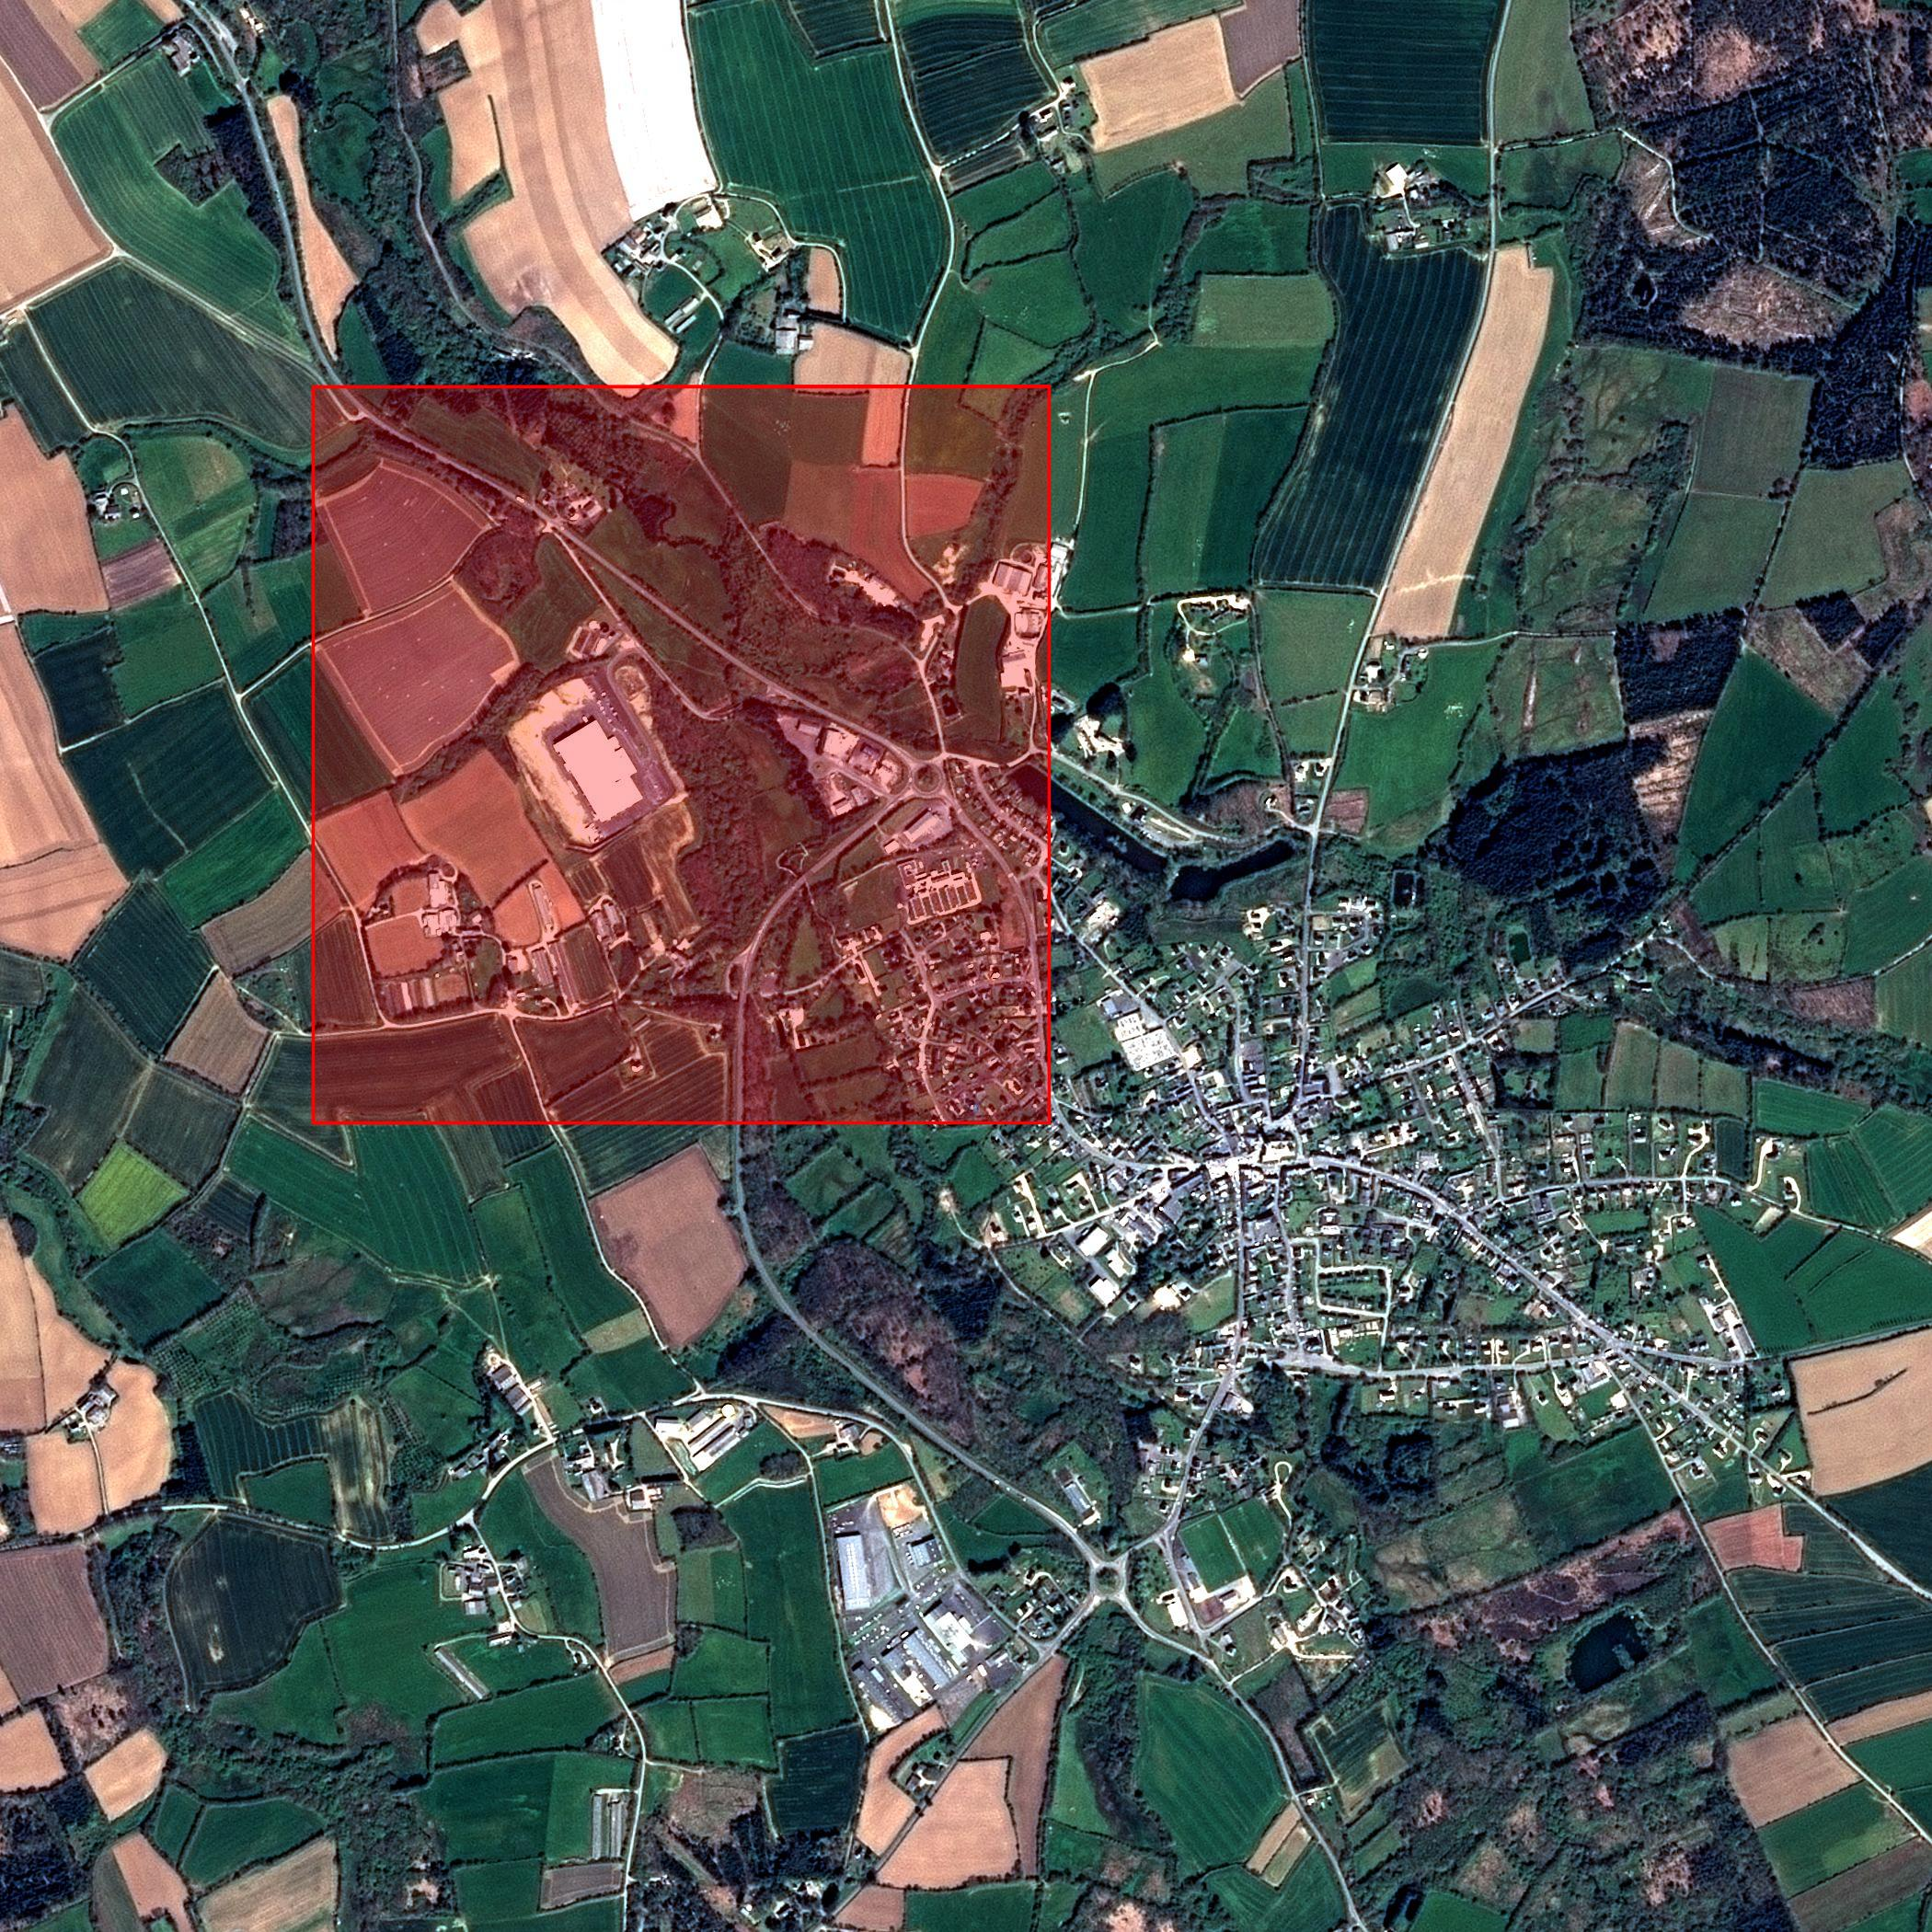
\includegraphics[width=.9\textwidth]{Im_SPOT6}
        \caption{Study area}
        \label{fig:areaBig}
    \end{subfigure}
    \hfill
    \begin{subfigure}{0.49\textwidth}
        \centering
        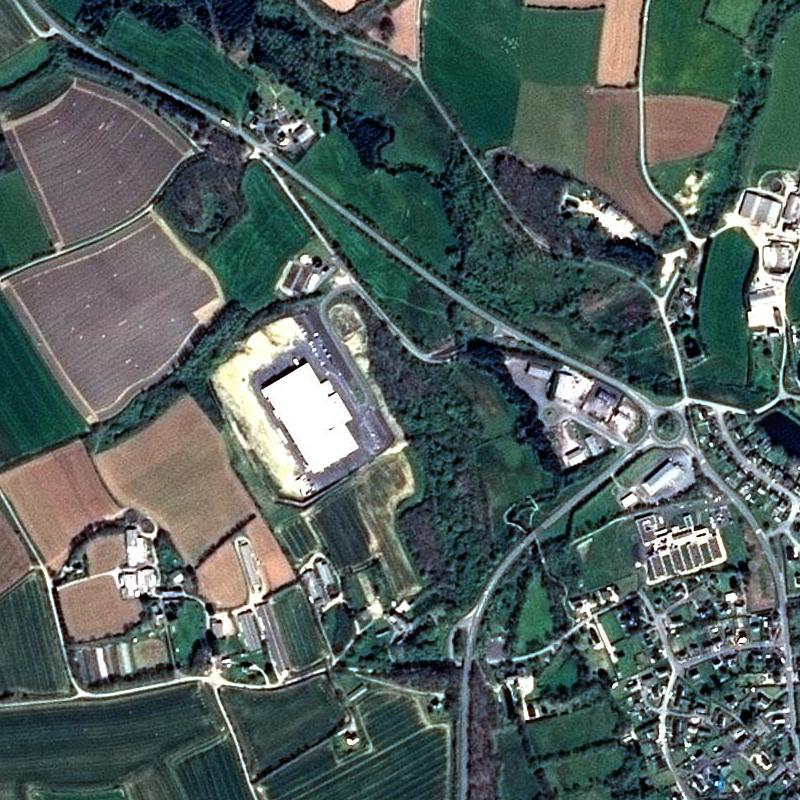
\includegraphics[width=.9\textwidth]{Im_SPOT6_crop}
        \caption{Crop window (800 $\times$ 800 m)}
        \label{fig:areaSmall}
    \end{subfigure}
    \caption{Study area and crop window}
    \label{fig:area}
    \centering
\end{figure}

\section{Methodology}\label{sec:method}
\subsection{Initial Fusion}

The data sets were first classified individually before fusion: The Sentinel-2 image was classified using all of its 13 bands (\textit{dates}) using a Random Forest classifier with \textit{50'000} samples \parencite{puissant_object-oriented_2014}. The SPOT-6 image was classified using a neural network described in \cite{postadjian_investigating_2017}.\\

Both classifiers produced 5 probabilities for the 5 classes proposed in the introduction (building, roads, water, forest and other vegetation).

\subsection{Fusion schemes}\label{sec:fusion}
% Notation to be used:
% TODO Explain better: Compromis WO, DS MasseSomme, DS MasseV1, Marge Bayes Pond / Marge Max / Marge Somme Pond / Moyenne  Bayes=Prod, Somme=Bayes Somme, CompromisWO=Walid Ouerghemmi

\subsubsection{Fuzzy Rules}\label{sec:fuzzyLogic}
The fuzzy rules presented below as well as the later presented Bayesian, Margin-based and Dempster-Shafer fusion rules are based on previous work by \cite{ouerghemmi_two-step_2017}. The first tested fusion approach is based on fuzzy rules \cite{zadeh_fuzzy_1965}. Fuzzy rule theory states that a fuzzy set $\mathcal{A}$ in a reference set $\mathcal{L}$ is a set of ordered pairs:
\begin{equation}
    A=[(x,P_A(x)|x\in \mathcal{L})]
\end{equation}
Where the membership probability of $A$ in $\mathcal{P}$ is given by $P_A:\mathcal{L}\rightarrow[0,1]$.

The measure of conflict between two sources ($1-K$) is given as (\cite{ouerghemmi_two-step_2017,dubois_possibility}):
\begin{equation}
    K=\sup_x\min(P_A(x), P_B(X))
\end{equation}
In order to account for the fact that fuzzy sets with a strong fuzziness possibly hold unreliable information, each fuzzy set $i$ is weighted by a confidence measure $w_i$ as proposed by \cite{fauvel_decision_fusion}:
\begin{equation}
    w_i=\frac{\sum_{k=0,k\neq i}^{n}H_{\alpha QE}(P_k)}{(n-1)\sum_{k=0}^{n}H_{\alpha QE}(P_k)}
\end{equation}
$n$ being the number of source and $H_{\alpha QE}$ a fuzziness measure called $\alpha$-quadratic entropy (QE) \parencite{pal_measuring_1994}. Every fuzzy set $i$ is weighted by the fuzziness degree of all other the other fuzzy sets (classifications) $k\in n,k\neq i$. If the fuzziness degree of the other sets is high the weight on a given source $i$ will be high too. For all of the following fusino rules, the fuzzy sets have been weighted as $P_A(x)=w_A\cdot\tilde{P}_A(x), P_B(x)=w_B\cdot\tilde{P}_B(x)$, $\tilde{P}_A(x)$ and $\tilde{P}_B(x)$ being the original membership probabilities and $w_A, w_B$ their corresponding pointwise measures.\\

The following fusion rules based on fuzzy logic were considered:
\begin{enumerate}
    \item Minimum rule as the intersection of two fuzzy sets $P_A$ and $P_B$, given by the minimum of their membership probabilities:
    \begin{equation}
        \forall A\in\mathcal{L} \;\;\; (P_A\cap P_B)(x) = P_{fusion}(x) =\min\big(P_A(x),P_B(x)\big)
    \end{equation}
    \item Maximum rule as the union between the two fuzzy sets $P_A$ and $P_B$, given by the maximum of their membership probabilities:
    \begin{equation}
        \forall A\in\mathcal{L} \;\;\; (P_A\cup P_B)(x) = P_{fusion}(x)=\max\big(P_A(x),P_B(x)\big)
    \end{equation}
    \item Compromise operator:
    \begin{equation}\label{eq:compro}
        P_{fusion}(x)=
        \begin{cases}
            \max\Big(T_1,\min\big(T_2,(1-K)\big)\Big)& \text{if } (1-K)\neq 0\\
            \max\Big(P_A(x),P_B(x)\Big) &\text{if }(1-K)= 1
        \end{cases}
    \end{equation}
    where $T_1=\frac{\min\big(P_A(x),P_B(x)\big)}{K}$ and $T_2=\max\big(P_A(x),P_B(x)\big)$, noticing that the operaor behavior is conjunctive when the conflict between $A$ and $B$ is low ($1-K\approx 0$) and disjunctive when the conflict is high ($1-K\approx 1$). When the conflict is partial, the operator behaves in a compromise way \parencite{ouerghemmi_two-step_2017}. This fusion approach would however favour $T_1$ at fusion level, therefore \cite{ouerghemmi_two-step_2017} propose to measure the intra-class conflict as $f_c=\abs(Cbest1-Cbest2)$ and set a conflict threshold $t_c=0.25$ to be used as follows:
    
    \begin{algorithm}[H]
        \begin{algorithmic}
            \If {$f_c<t_c$} 
            \Comment{existence of intra-membership conflict}
            \State $P_{fusion}=\max\big(P_A(x),P_B(x)\big)$
            \Else
            \Comment{no intra-membership conflict}
            \State $P_{fusion}$ following equation \ref{eq:compro}
            \EndIf
        \end{algorithmic}
        \caption{Compromise rule according to \cite{ouerghemmi_two-step_2017}}
        \label{alg:comp-wo}
    \end{algorithm}
    \item Prioritized operators (Prior 1, eq. \ref{eq:prior1} and Prior 2, eq. \ref{eq:prior2}):
    \begin{align}
        P_{fusion}(x)&=\max\big(P_A(x),\min(P_B(x),K)\big)\label{eq:prior1}\\
        P_{fusion}(x)&=\min\Big(P_A(x),\max\big(P_B(x),(1-K)\big)\Big)\label{eq:prior2}
    \end{align}
\end{enumerate}

\subsubsection{Bayesian combination}\label{sec:bayesian}
A very simple approach is to sum or multiply the input probabilities as a Bayesian sum or product:
\begin{align}
    P_{fusion}&=P_A(x)+P_B(x)\\
    P_{fusion}&=P_A(x)\times P_B(x)
\end{align}
\subsubsection{Margin-based Rule (Margin-Max)}\label{sec:margin}
In the Max-Margin approach, the aim is to conserve the the most confident source in each pixel, that is, the one having the least smallest margin:
\begin{equation}
    margin^{(s)}(x)=P_s^{cbest1}-P_s^{cbest2}(x)
\end{equation}
where $cbest1=\argmax_{c\in\mathcal{L}}P_S(C)$ and $cbest2=\argmax_{c\in\mathcal{L}\setminus cbest1}P_S(C)$. The fusion will choose for each pixel the source for which the margin between the two highest probabilities is the biggest, with sources $\mathcal{S}={A,B}$ and the classes $\mathcal{L}=\{\mathcal{C}_i\}_{i\in[1,n]}$:
\begin{equation}
    \forall x,\forall c\in \mathcal{L}\;\;\; P_{fusion}^{(c)}(x)=P_{S_{best}}^{(c)}(x)
\end{equation}
where $S_{best}=\argmax_{\mathcal{S}\in\mathcal{C}}margin^{(s)}(x)$.


\subsubsection{Dempster-Shafer (DS) evidence theory}\label{sec:DS}
According to the DS formalism, an information from a source $s$ for a class $c$ can be given as a mass function $m_c\vert m_c\in [0,1]$ (\cite{shafer-evidence}). Dempster-Shafer's evidence theory rule assumes simple classes $c\in \mathcal{L}$ as well as composed classes, which were limited to at most two simple classes as indicated in \cite{ouerghemmi_two-step_2017}. Masses associated to each simple class were denoted as taking simply the pointwise class membership probability.
\begin{align}
    m_s^{(c)}(x)=P_s^{(x)}
\end{align}
For compound classes, $\forall c1,c2\in \mathcal{L}, \forall$ pixel $x$ and $\forall s\in \mathcal{S}$:
\begin{equation}
    m_s^{(c1\cup c2)}(x)=\big(P_s^{(c1)}(x)+P_s^{(c2)}(x)\big)\times \Big(1-\max\big(P_s^{(c1)}(x),P_s^{(c2)}(x)\big)\Big)+\min\big(P_s^{(c1)}(x),P_s^{(c2)}\big)
\end{equation}
This yields a mass $m_s^{(c1\cup c2)}(x)\in [0,1]$ being 1 if $P_s^{(c1)}=0, P_s^{(c2)}=1$ or $P_s^{(c2)}=0, P_s^{(c1)}=1$. All masses are normalized such that $\sum_{c \in \mathcal{L}}^{(s)}m_c^{(s)}(x)=1$.
The fusion rule is based on the following conflict measure between two sources $A$ and $B$:
\begin{align}
    k(x)=\sum_{\substack{c,d\in\mathcal{L}'\\c\cap d\neq\emptyset}}^{(s)}=m_A^{(c)}(x)m_B^{(c)}(x)
\end{align}
$c,d\in\mathcal{L}$ being compound classes with $c\cap d =\emptyset$. The fusion is performed as:
\begin{equation}
    m_{fusion}^{(c)}(x)=\frac{1}{1-k(x)}\sum_{\substack{c1,c2\in\mathcal{L}'\\c1 \cap c2 = c}}^{(s)}m_A^{(c)}(x)m_B^{(c)}(x)
\end{equation}

\subsubsection{Fusion by Classification}
Supervised Classification Methods were used to train a model on the ground truth available from the BDTOPO (\textit{reference}) database, using the LIBSVM and Open CV libraries (\cite{libsvm,opencv}). The following three models were tested:  % TODO Put reference
% TODO test filling gaps with roads
\begin{enumerate}
    \item Random Forest (RF), with 10'000 training samples (\cite{opencv})
    \item Support Vector Machine (SVM) with a linear kernel ($u'\times v$), with 10'000 training samples (\cite{libsvm})
    \item Support Vector Machine with a radial basis function: $\exp(-\gamma*|u-v|^2)$ (\cite{libsvm})
\end{enumerate}

\subsection{Weighting}
All methods above have been tested using the original class probabilities as input  as well as using the probabilities weighted by the pointwise measure of their fuzziness degree (section \ref{sec:fuzzyLogic}). The hypothesis was that weighting the probabilities by their fuzziness could help improve other fusion methods as well by reducing the importance of fuzzy sources. In fig. \ref{fig:proba_point}, an example is shown where the SPOT 6 classifier has a higher fuzziness degree than the Sentinel-2 classifier, hence the probability of the SPOT 6 classifier is reduced more strongly by the pointwise measure.

\begin{figure}[H]
    \centering
    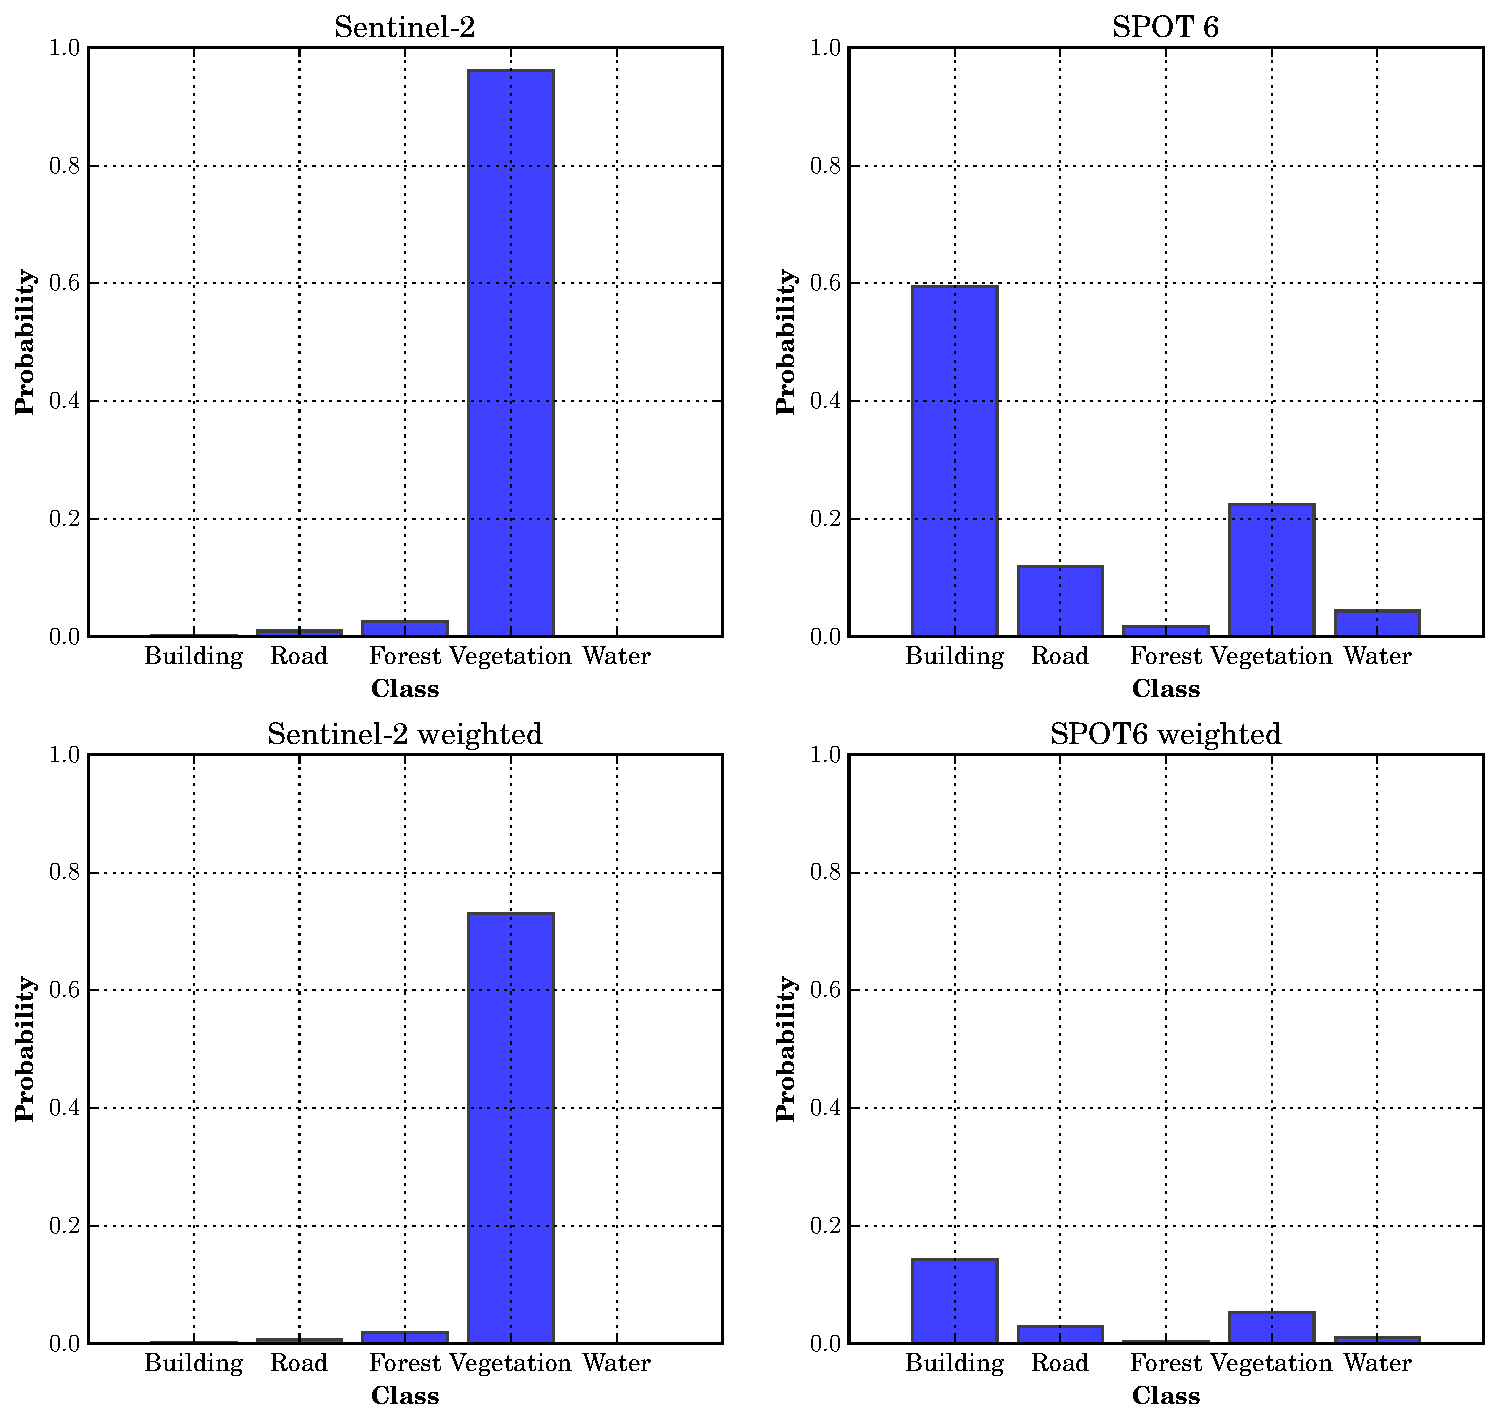
\includegraphics[width=.7\textwidth]{proba_point}
    \caption{Original and weighted class probabilities}
    \label{fig:proba_point}
\end{figure}


\subsection{Regularization}\label{sec:regularization}
In order to smooth the fusion result, which still contains noisy patches, and make it follow real-world contours more accurately, a  energy minimization regulation function was applied based on previous work by \cite{hervieu_fusion_2016} and \cite{ouerghemmi_two-step_2017}. The regularization consists of two terms, one attached to the data, and one to the regularization respectively:

\[E(P_{fusion},C_{fusion},C)=\sum_{x\in I_{MS}}E_{data}(C(x))+\lambda\sum _{\substack{x,y\in N\\x\neq y}}E_{reg}(C(x),C(y)) \]
where:
\begin{align}
E_{data}\big(C(x)\big)&=f\Big(P_{fusion}C(x)\big)\Big)\\
E_{reg}\big(C(x)=C(y)\big)&=g\Big(P_{fusion}\big(C(x)\big),C_{fusion}\Big)\\
E_{reg}\big(C(x)\neq C(y)\big)&=h\Big(P_{fusion}\big(C(x)\big),C_{fusion}\Big)
\end{align}
The data term is a fit-to-data attachment term which models the probability distribution $P_{fusion}$. defined by a function $f(t)$. Following options were tested:
\begin{align}
f(t)&=-\log(x)
f(t)&=1-x
\end{align}
The regularization term $E_{reg}$ was decomposed into two component, one being a Pott's model to prefer smoother label changes and a term attached to contrast in the original image.
\begin{align}
    E_{reg}(C(x)=C(y)&=0\\ 
    E_{reg}(C(y)\neq C(y))&=(1-\gamma)+\gamma V(x,y,\varepsilon)
\end{align}
With $\gamma = 0$ yielding a pure Potts model and $\gamma = 1$ putting all weight on the contrast term. The contrast component accounts for the fact that label changes need not be penalized at strong contrast changes. Two alternative models were compared:
$V(x,y,\varepsilon)$ being the term for contrast
\begin{enumerate}
    \item Option 1, based on \cite{ouerghemmi_two-step_2017}: 
    \begin{equation}
        V(x,y)=\frac{1}{dim}\sum_{i\in[0,dim]}V_i(x,y)^\varepsilon
    \end{equation}
    Where $V_i(x,y)=\exp\Bigg(\frac{-\big(I_i(x)-I_i(y)\big)^2}{2\big(\overline{I_i(x)-I_i(y)}\big)^2}\Bigg)$
    \item Option 2, based on \cite{schindler_overview_2012}:
    \begin{equation}
        \begin{aligned}
            &\mathcal{G}_{0.5}\odot
            \begin{bmatrix}
            -1 &1
            \end{bmatrix}& \mathcal{G}_{0.5}\odot
            \begin{bmatrix}
            1 \\
            -1
            \end{bmatrix}&\\
            &\mathcal{G}_{0.5}\odot
            \begin{bmatrix}
            -1 & 0 \\
            0 &-1
            \end{bmatrix}&\mathcal{G}_{0.5}\odot
            \begin{bmatrix}
            0& 1 \\
            -1 &0
            \end{bmatrix}&\\
        \end{aligned}
    \end{equation}
    For example, the gradient in the horizontal row would be $\dot{I}=||\mathcal{G}_{0.5}\odot\begin{bmatrix}-1 &1\end{bmatrix}\odot I||$. The contrast term penalizes label changes most strongly if the contrast is zero, and decreases linearly until a point where it becomes zero, for which $\phi=70\%$ is chosen. The contrast formula thus writes:
    \begin{equation}
        E_{smooth}(C(u)\neq C(v))=\max\Big(0,1-\frac{2-\phi}{\dot{I}_{MAX}}\dot{I}_{u\rightarrow v}\Big)
    \end{equation}
\end{enumerate}
For both contrast alternatives, a large number of combinations of values were tested on a small test zone and narrowed than successively to reach the best combination. Cross-validation between parameters was performed to find the best values for $\lambda$ $\gamma$ and $\varepsilon$ yielding the nicest and smoothest possible result while following the real object contours.\\

In addition, the image used for the contrast term was dilated by a Gaussian filter of standard deviation 2, which helped smoothen the regulation output.

\subsection{Binary classification}
The class probabilities from the initial classifications on the original images and the class probabilities from the regularization step were aggregated such as to obtain two classes, one for artificialized areas ($a$) and one for non-artificialized areas ($\neg a$), such as:
\begin{align}
    P(a)=P(b)+P(r),  &\;P(\neg a)= 1 - P(a)
\end{align}
$P(b)$ and $P(r)$ being the class probabilities for buildings and road respectively, given the classes $b, c\in \mathcal{C}$  and $\sum_{c \in \mathcal{C}}P(c) = 1 $.

\subsection{Artificialized area}
The binary class probabilities were used to perform a second fusion of the regularization result with the Sentinel-2 classification in order to find the extent of the urban tissue, consisting of contiguous structures of buildings and roads on a coarser level. Two methods were tested:\\

% Regularization modifications
Firstly, the binary class probabilities were extracted. A linear decreasing function assigning a probability from 1 to 0 to be in an artificialized area was applied surrounding all buildings, reaching a probability of 0 to be in an artificialized area after a distance of 200 meters.
%TODO show probability dilatation steps
This probability map together with binary class probabilities from the Sentinel-2 classifier are used for fusion and regularization, using the Min rule and the same parameters for regularization as described above.\\

% Segmentation
Secondly, a segmentation on the Sentinel-2 image has been performed to use majority voting of the dilated binary regulation result just described to determine the class labels in the segmented image regions. Segmentation is performed using the "scale climbing" algorithm described in \cite{guigues_scale-sets_2003} and repeated with cuts of 3, 8, 20 and 30.

\subsection{Evaluation}

Evaluation was performed on the fusion and regularization results on all five classes, applied to 5 tiles of 3000 $\times$ 3000m size, totalling an area of 45 $km^2$. The class labels of each classification were compared against the class labels of the ground truth of the freely available BD TOPO database, from which a ground truth map of 5 class labels was derived (\cite{bdtopo}, fig. \ref{fig:vt}).

\begin{figure}[H]
    \centering
    \begin{subfigure}{0.49\textwidth}
        \centering
        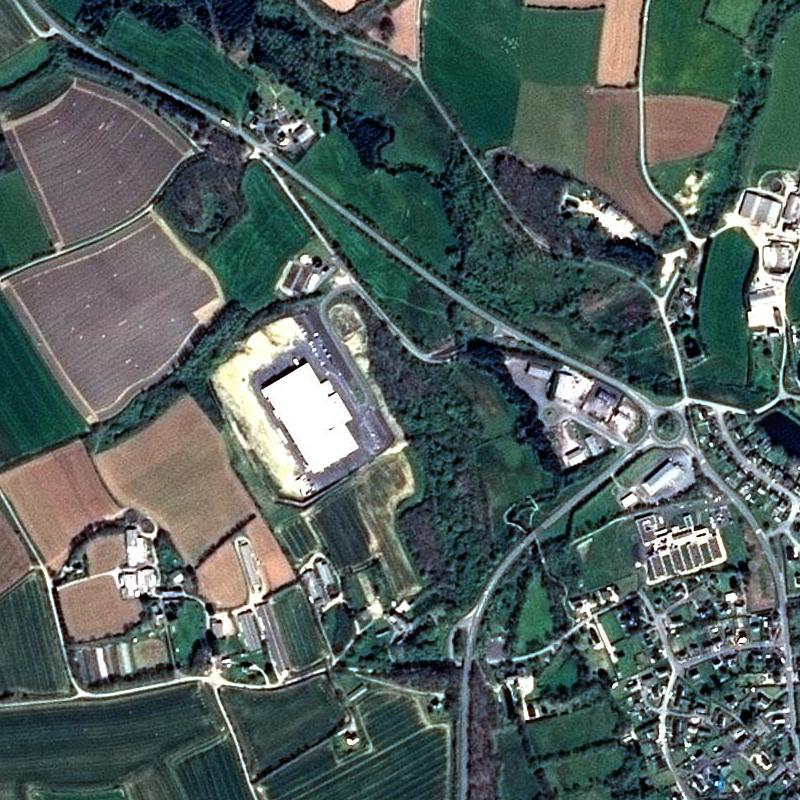
\includegraphics[width=\textwidth]{Im_SPOT6_crop}
        \caption{Original image (SPOT 6)}
        \label{fig:SPOT6}
    \end{subfigure}
    \begin{subfigure}{0.49\textwidth}
        \centering
        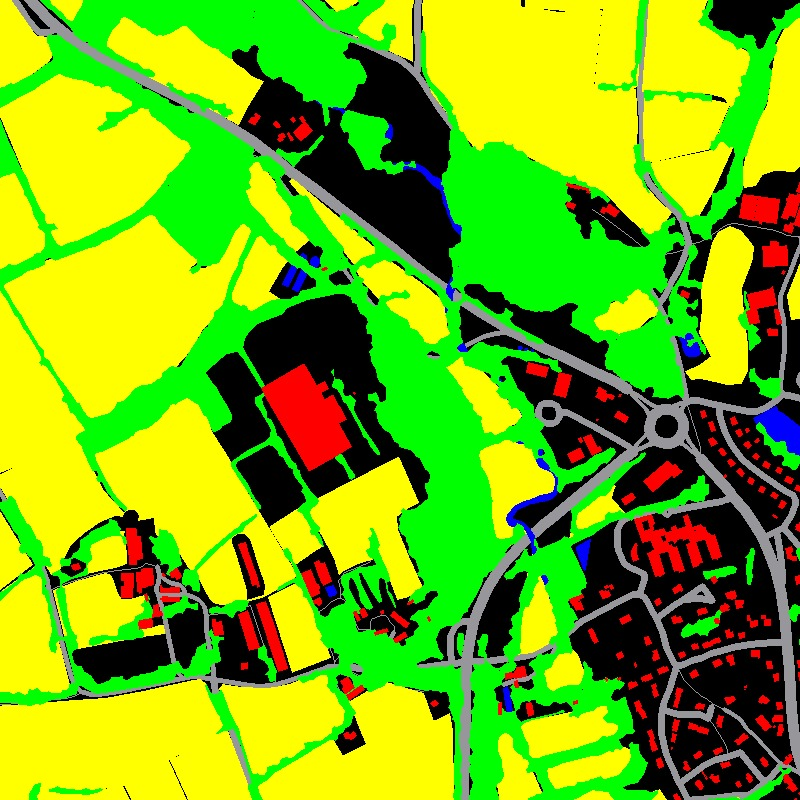
\includegraphics[width=\textwidth]{T41000_30000_train}
        \caption{Ground Truth}
        \label{fig:GT}
    \end{subfigure}
    \legende
    \caption{Original image and ground truth. Black parts indicate missing ground truth data.}
    \label{fig:vt}
\end{figure}



Following indicators were produced for each classification (\cite{deMorsier}):
\begin{itemize}
    \item Overall Accuracy (OA) and User Accuracy (UA) scores based on Confusion matrices, illustrated with two classes in table \ref{table:cm}.
    \begin{table}[H]
		\centering
		\begin{tabular}{cc|c|c|cl}
			& & \multicolumn{2}{l|}{True labels y}&PA\\
			\multirow{3}{*}{Predicted labels y} &  & O& B  &\\ \cline{1-5} 
			& O &  $n_{OO}$ & $n_{OB}$ &$n_{OO}/n_{O\bullet}$\\ \cline{2-5} 
			& B & $n_{BO}$ & $n_{BB}$  &$n_{BB}/n_{B\bullet}$\\ \cline{1-5} 
			\multicolumn{2}{c|}{UA} & $n_{OO}/n_{\bullet O}$ & $n_{BB}/n_{\bullet B}$&OA$=\sum_in_{ii}/n_{\bullet\bullet}$\\
		\end{tabular}
		\caption{Confusion matrix: UA = User's Accuracy, PA = Producer's Accuracy, OA = Overall Accuracy, B=Building, O=Other. Bullets indexes signify either the sum of the row (e.g., $n_{O\bullet}$), the sum of the column (e.g., $n_{\bullet O}$) or the sum of all elements of the confusion matrix ($n_{\bullet\bullet}$).}
		\label{table:cm}
	\end{table}
	\item Cohen's Kappa:
	\begin{equation}
	    \kappa=\frac{P_{obs}-P_{est}}{1-P_{est}},P_{obs}=OA=\frac{\sum_in_{ii}}{n}, P_{est}=\frac{\sum_i\big(\frac{\sum_jn_{ij}\sum_jn_{ji}}{n}\big)}{n}
	\end{equation}
	\item F-Score, as a weighted harmonic measure between the precision and the recall:$     F1=\frac{2PR}{P+R}$
    The mean F-Score over all classes and the F-Scores specifically for the buildings class are indicated. Methods are ranked with respect to their AA and F-Scores for the buildings class.
\end{itemize}


\subsection{Workflow}
Figure \ref{fig:methods} shows the overall workflow for producing a classification based on fusion, regularization as well as the second classification using the Sentinel2 image, illustrating all the above-mentioned steps. The fusion method producing the best results in terms of visual quality, absence of artifacts and accuracy measures was retained and used further in the Regularization step. Several regularization parameters mentioned above were tested and the set of parameters producing the best map was retained, again in terms of its visually appealing properties, truthfulness to the real-world objects and evaluation with respect to the ground truth.

\begin{figure}[H]
    \centering
    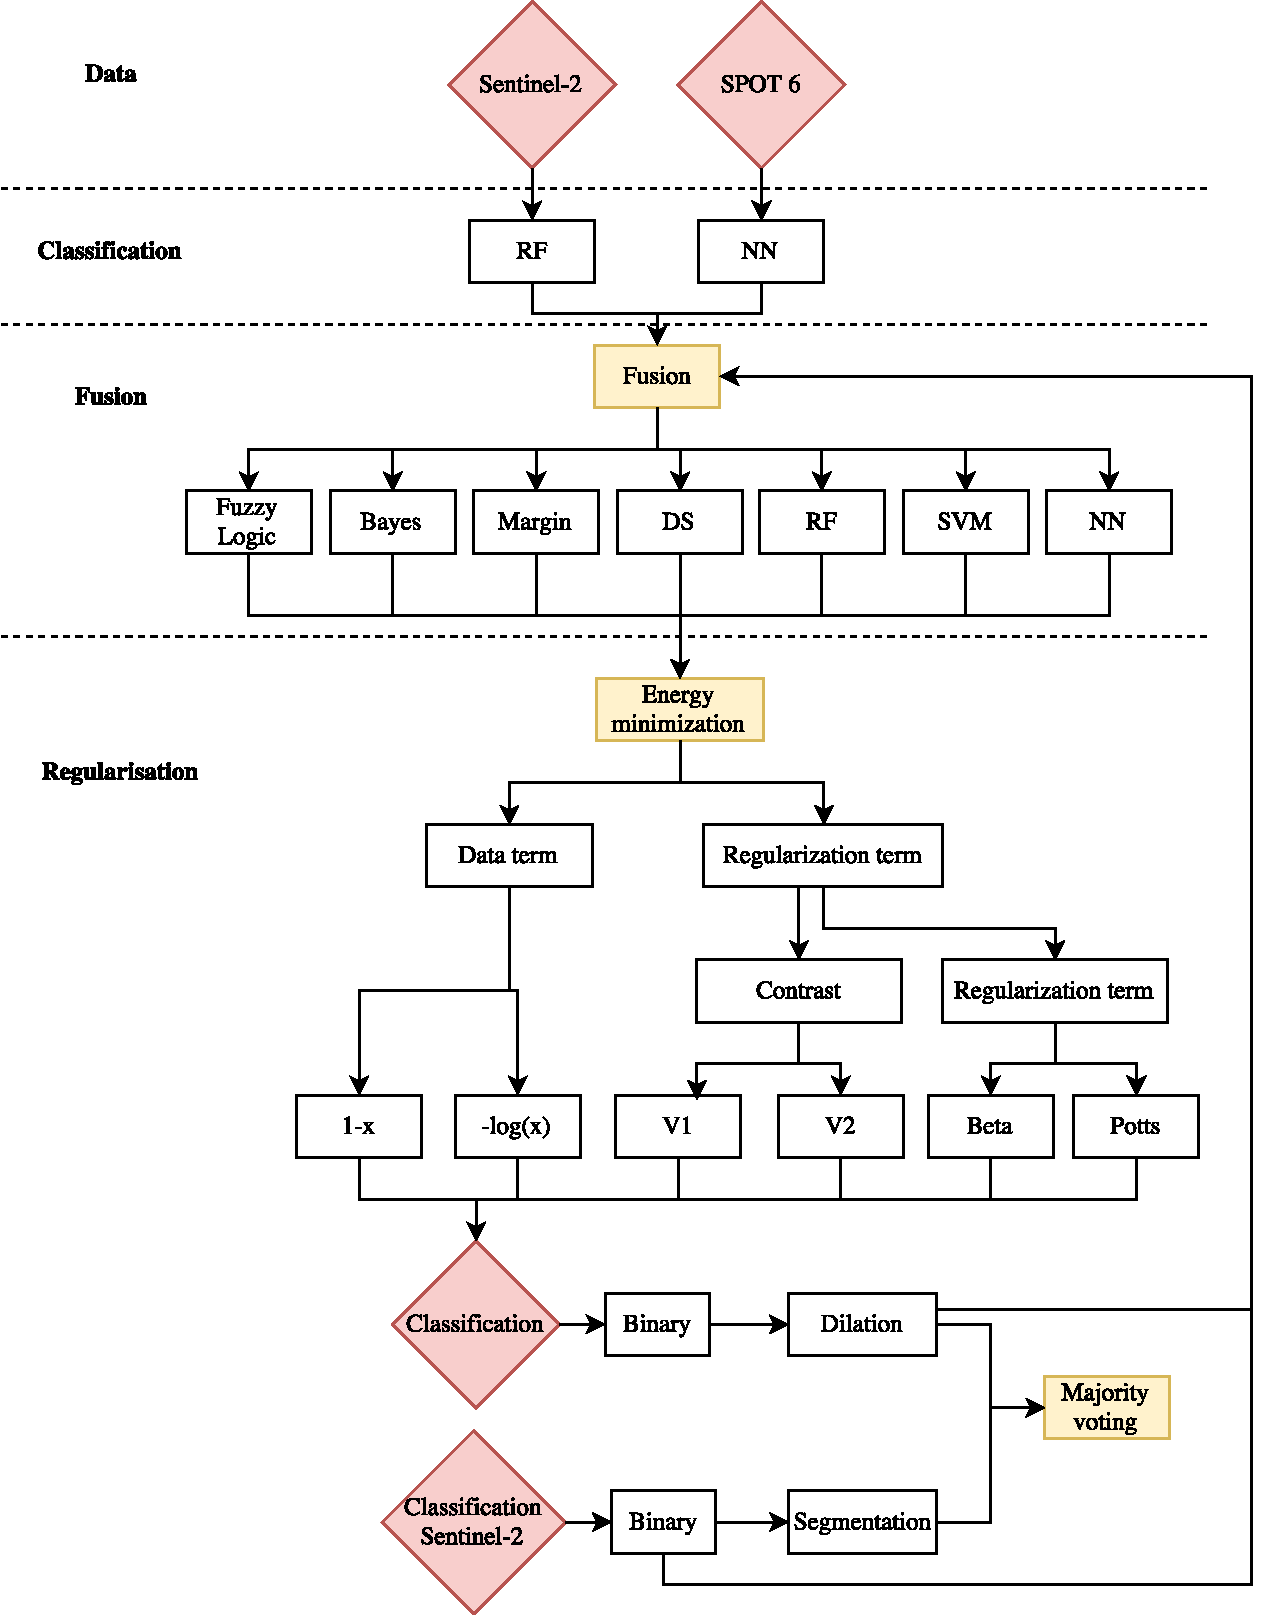
\includegraphics[width=.7\textwidth]{IGN-methods}
    \caption{Methods}
    \label{fig:methods}
\end{figure}

\newpage

\section{Results}
\subsection{Original Classifications}
The original classification confirms well the initial observation that the SPOT6 classifier tends to badly classify certain parts, while preserving geometries, while the S2 classifier overall behaves better, while mixing buildings and roads due to its coarse spatial resolution. Figure \ref{fig:cl_orig} shows the original classification result from the individual classifications on the SPOT 6 and Sentinel-2 images as well as the original image and ground truth.\\

A few particularly interesting confusions can be highlighted:
\begin{enumerate}
    \item The SPOT6 classifier discovers a big patch of buildings and road in the top-left corner where there is actually a field (probabilities are shown in fig. \ref{fig:proba_point}). This is probably due to the fact that the field was barren at the time the image was taken and leads to a wrong classification due to the low number of bands. The patch is correctly labelled in the Sentinel-2 classification.
    \item In the middle of the image, there is an industrial complex visibly surrounded by roads and concrete ground. Several patches around the building are wrongly classified as water by the SPOT 6 classification while there is also a minor however smaller amount of confusion in Sentinel-2.
    \item Individual buildings in the left-hand corner are nicely recognizable in the SPOT 6 classification, and they are mixed with the roads in the Sentinel-2 classification due to its lower resolution.
\end{enumerate}

\begin{figure}[H]
    \centering
    \begin{subfigure}{0.49\textwidth}
        \centering
        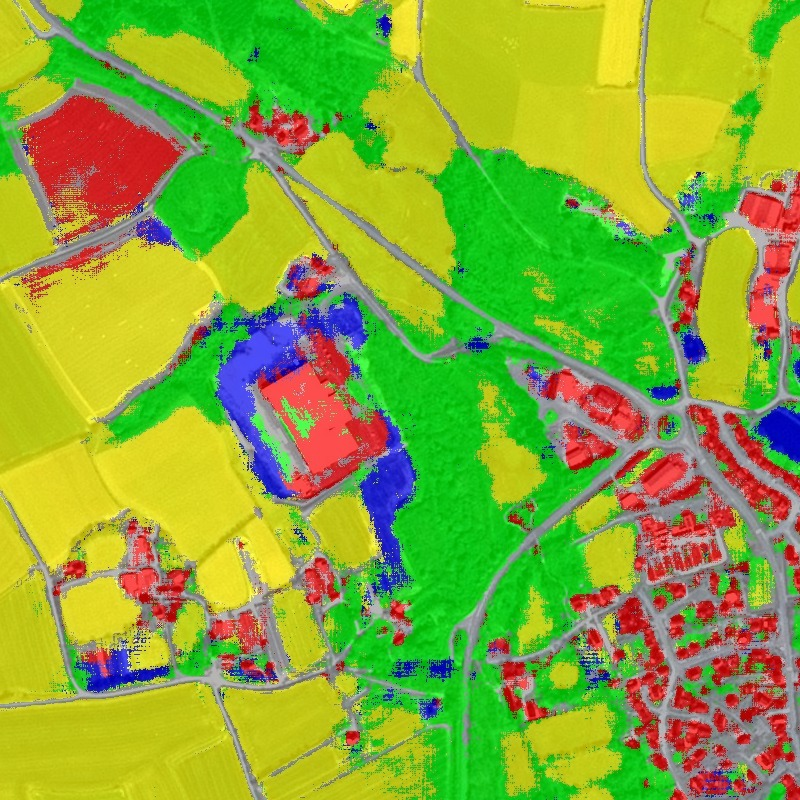
\includegraphics[width=.9\textwidth]{T41000_30000_classif_SPOT6_all}
        \caption{SPOT 6 classification}
        \label{fig:SPOT6cl}
    \end{subfigure}
    \begin{subfigure}{0.49\textwidth}
        \centering
        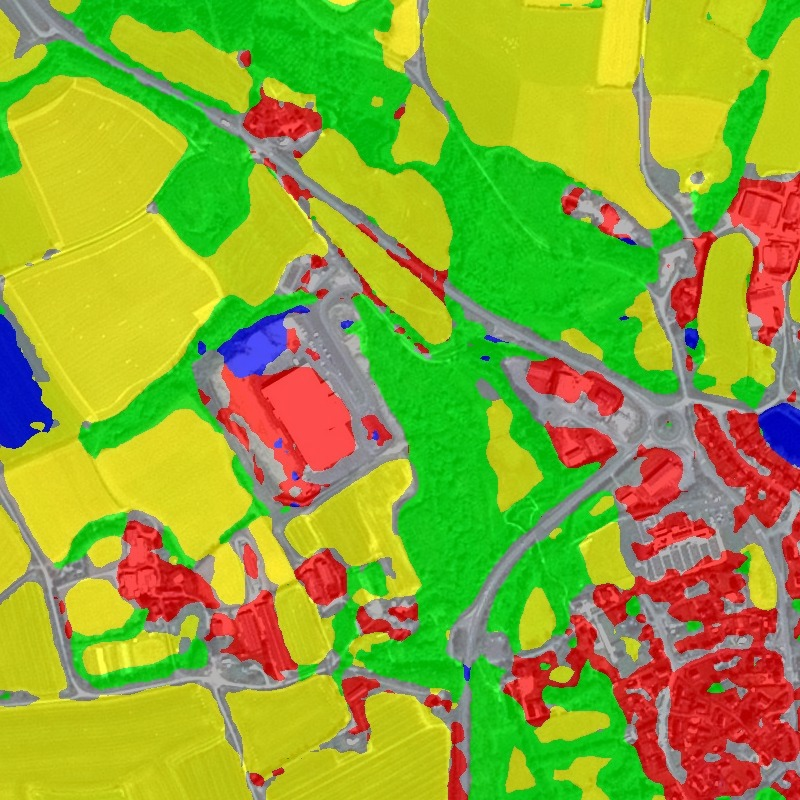
\includegraphics[width=.9\textwidth]{T41000_30000_classif_S2_all}
        \caption{Sentinel 2 classification}
        \label{fig:S2cl}
    \end{subfigure}
    \legende
    \caption{Original image, ground truth and classifications. The SPOT6 image is superposed transparently in the background of the classifications. }
    \label{fig:cl_orig}
\end{figure}



\subsection{Fusion}
All results of the fusion are shown in appendix \ref{app:subsec:fusion}. The Min and Bayes classifiers were produced the best results since they followed the objects most precisely while producing the least class confusions (fig. \ref{fig:fusion}).

\begin{figure}[H]
    \centering 
    \begin{subfigure}{0.49\textwidth}
        \centering
        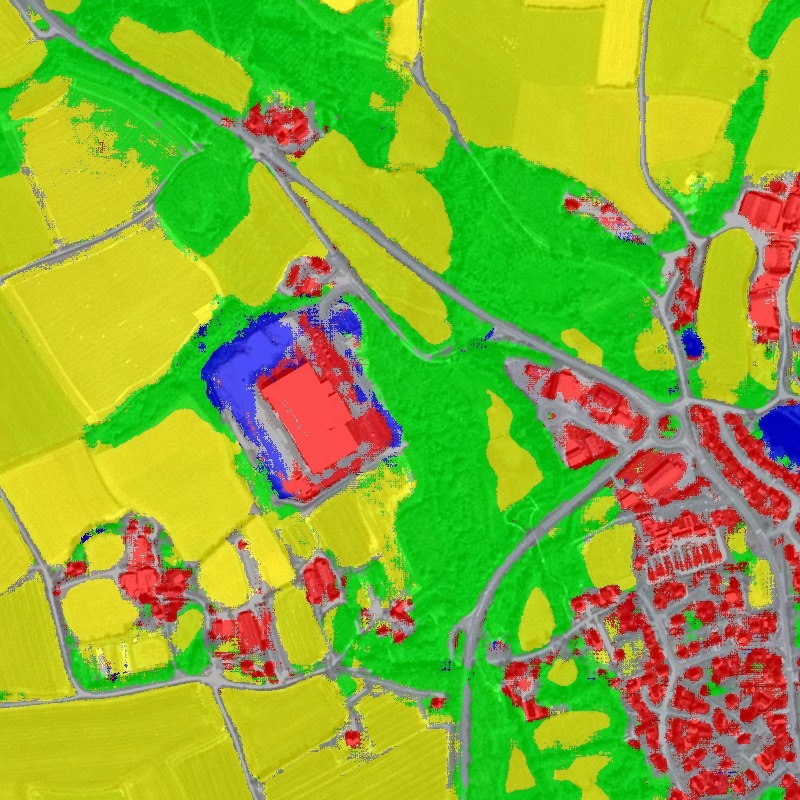
\includegraphics[width=\textwidth]{T41000_30000_classif_Fusion_Min_weighted}
        \caption{Fusion: Min}
        \label{fig:fusion_min}
    \end{subfigure}
    \begin{subfigure}{0.49\textwidth}
        \centering
        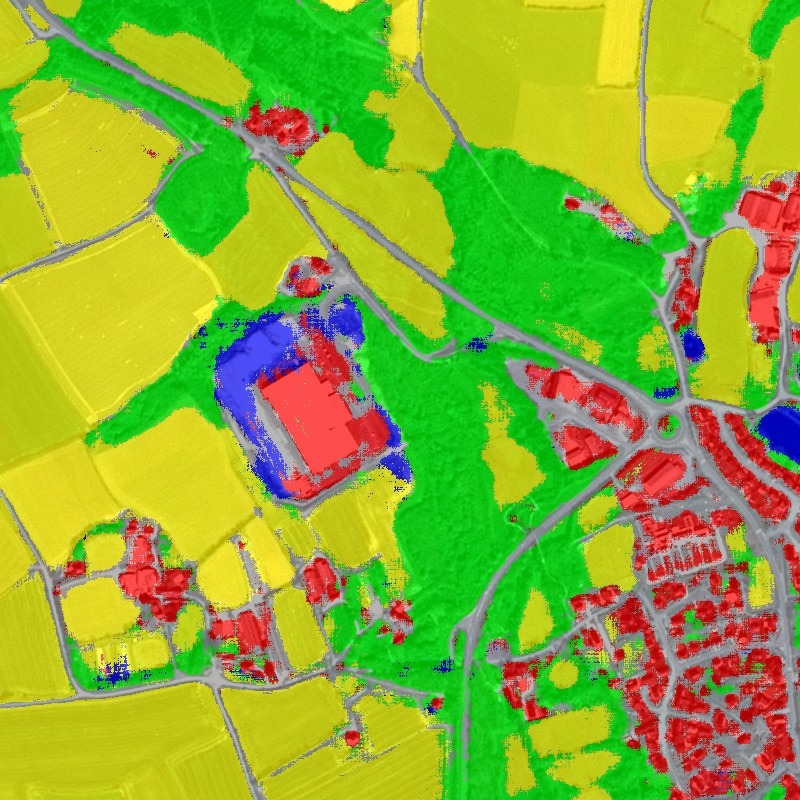
\includegraphics[width=\textwidth]{T41000_30000_classif_Fusion_Bayes_weighted}
        \caption{Fusion: Bayes}
        \label{fig:fusion_bayes}
    \end{subfigure}
    \legende
    \caption{Original image, ground truth and classifications.}
    \label{fig:fusion}
\end{figure}


Although these classifiers are amongst the mathematically most simple, they produced clearly better results than more complex models such as the Prior rule or the Compromise rule (appendix \ref{app:subsec:fusion}). Evaluation numbers for the Min and Bayes classifier were also consistently higher (table \ref{table:eval}).\\

With respect to the comments on the individual classifications before fusion:
\begin{enumerate}
    \item Both classifiers manage to get rid of the wrongly classified building patch in the top-left corner (cf. fig. \ref{fig:SPOT6cl}), preferring the Sentinel-2 classification pixels over the one of SPOT6. However, the Bayesian classifier follows the field contours more smoothly than the Min classifier. % TODO show pixel values
    \item The industrial zone in the middle is still confused with water in both classifiers, however the southeastern part of it is now correctly classified as vegetation.
    \item Both classifiers manage to conserve the level of detail within the urban patch in the bottom-right corner. However, a closer look reveals that the Min classifier preserves more detail in densely populated areas while the Bayes classifier has a slightly higher tendency to connect buildings within patches. 
\end{enumerate}
Due to the last reason, the Min classifier was further used for regularization in order to keep buildings apart.

\subsection{Regularization}

The model and parameters chosen for the final regulation are as follows:
\begin{itemize}
    \item Data term: $f(t)=1-x$ since a logarithmic model would penalize too strongly locally bad classifications (the energy terms rises to $\infty$ as $x\rightarrow 0$).
    \item Contrast model 1, since model 2 was not enough adaptable (behaved very similar under different parameter sets and did not show significant improvement over model 1)
    \item Optimal parameters: $\lambda = 10, \gamma = 0.7, \varepsilon = 50$
\end{itemize}
The regulation product using the above-mentioned regulation model and parameters is shown in figure \ref{subfig:regularisation}.
\begin{figure}[H]
    \centering 
    \begin{subfigure}{0.49\textwidth}
        \centering
        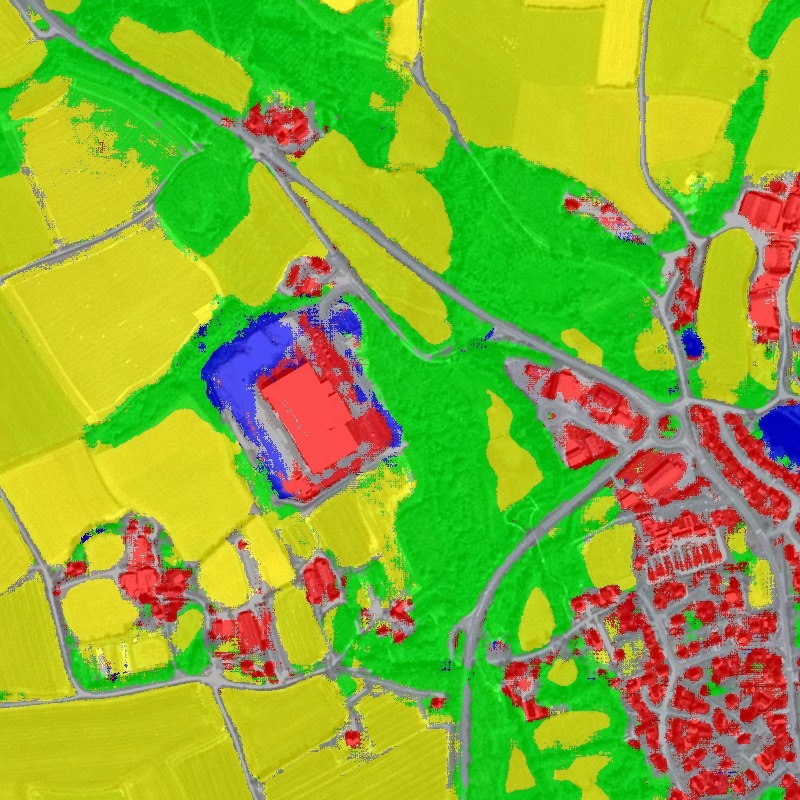
\includegraphics[width=\textwidth]{T41000_30000_classif_Fusion_Min_weighted}
        \caption{Fusion}
        \label{subfig:fusion_min}
    \end{subfigure}
    \begin{subfigure}{0.49\textwidth}
        \centering
        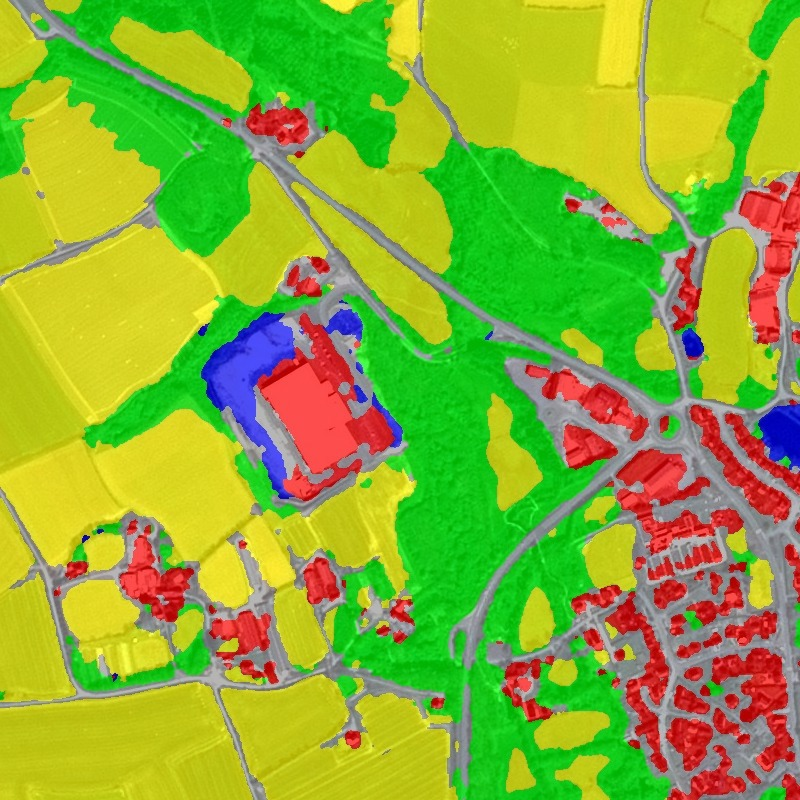
\includegraphics[width=\textwidth]{T41000_30000_regul_Min_weighted_G2_l1000_g70_e500_0_0_0}
        \caption{Regularization}
        \label{subfig:regularisation}
    \end{subfigure}
    \legende
    \caption{Fusion and Regularization of the Min Classifier}
    \label{fig:fusion_regularisation}
\end{figure}
The regulation does its job smoothing out small noisy patches and yielding a visually more appealing result, although its evaluation numbers are lower compared to those of the fusion (cf. table \ref{table:eval}).

\subsection{Artificialized area}
\subsubsection{Fusion with Sentinel-2}
Results using the dilated binary class probabilities from the regulation and the binary Sentinel-2 class probabilities are shown in figure \ref{fig:regul_fusion}.
\begin{figure}[H]
    \centering
    \foreach \n/\captiontext in {classif_regul_urbain/Input: Dilated binary regulation result,
    classif_S2_urbain/Input: Sentinel-2 binary classification,
    classif_Fusion_Min/Fusion by Min rule,
    regul_proba_Fusion_Min_100_1000_100_0_100_70_100_200_0_0_0/Regulation
    }{
    \begin{subfigure}{0.49\textwidth}
        \centering
        \includegraphics[width=.9\textwidth]{R2_T41000_30000_\n}
        \caption{\captiontext}
    \end{subfigure}
    }
    \legendebin
    \caption{Artificialized Area: Input data, Fusion and Regularization}
    \label{fig:regul_fusion}
\end{figure}

\subsubsection{Segmentation}
Results using majority vote of the dilated binary class probabilities within the segmented image regions of Sentinel-2 are shown in figure \ref{fig:regul_fusion}. 
\begin{figure}[H]
    \centering
    \foreach \n/\captiontext in {3,8,20,30}{
    \begin{subfigure}{0.49\textwidth}
        \centering
        \includegraphics[width=.9\textwidth]{regul_seg_maj_\n}
        \caption{cut=\n}
    \end{subfigure}
    }
    \legendebin
    \caption{Segmentation}
    \label{fig:segmentation}
\end{figure}
A higher cut value leads to lesser and on average bigger segmented sub-regions and thus greater generalization of the area. 

\subsubsection{Comparison}
\begin{figure}[H]
    \centering
    \begin{subfigure}{0.49\textwidth}
        \centering
        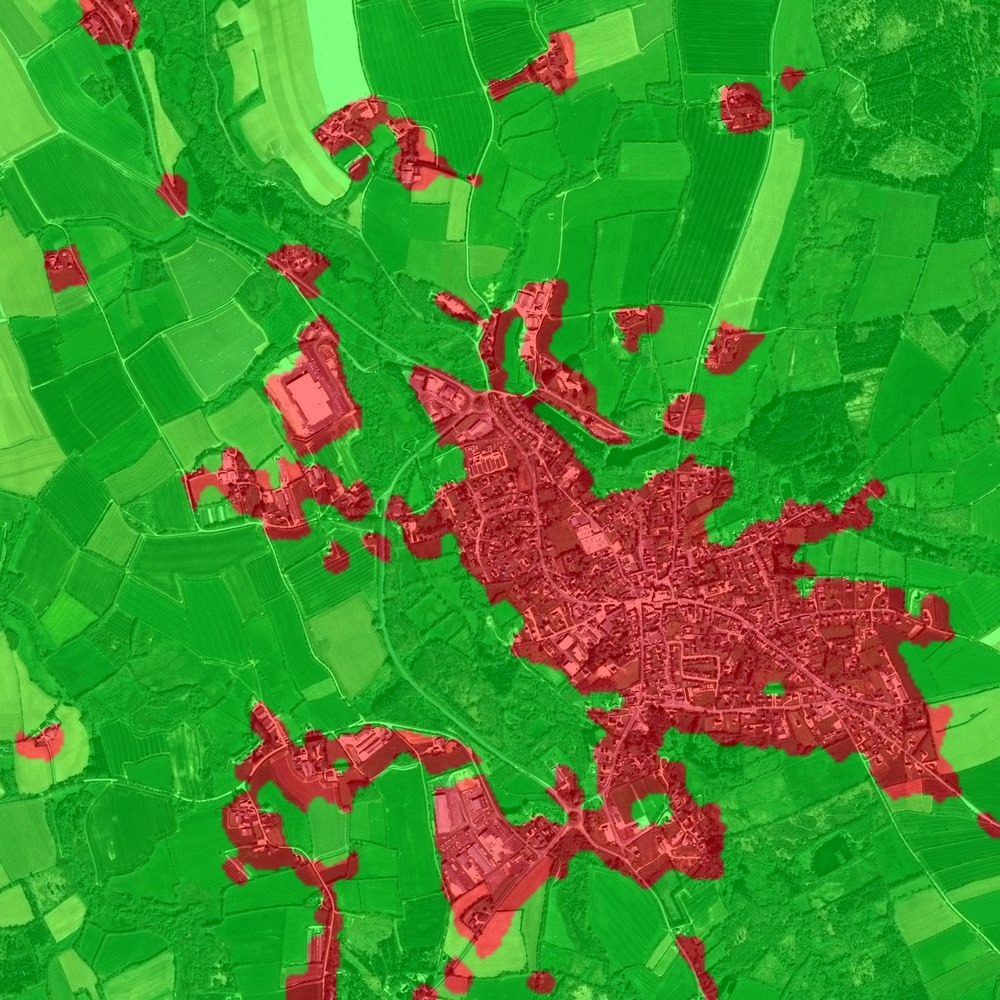
\includegraphics[width=\textwidth]{R2_T41000_30000_regul_proba_Fusion_Min_100_1000_100_0_100_70_100_200_0_0_0}
        \caption{Fusion and Regularization}
        \label{subfig:fusionRegComp}
    \end{subfigure}
    \begin{subfigure}{0.49\textwidth}
        \centering
        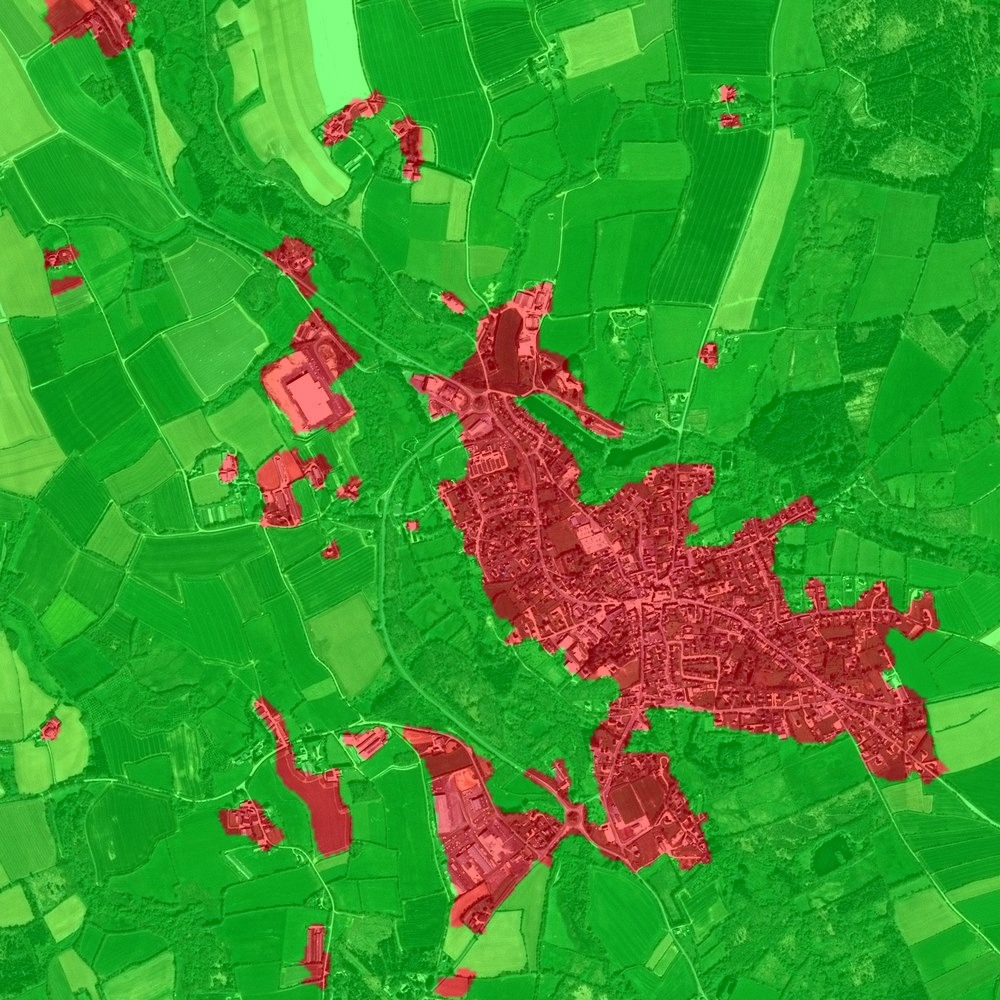
\includegraphics[width=\textwidth]{regul_seg_maj_20}
        \caption{Segmentation with CUTS=20}
    \end{subfigure}
    \legendebin
    \caption{Comparison between fusion and segmentation}
    \label{fig:comparison}
\end{figure}
While the fusion and regulation gives a more smoothed and visually appealing result, the segmentation shows a substantial number of improvements over the simple fusion with the Sentinel-2 classification:
\begin{itemize}
    \item It provides a more accurate classification in terms of following the original image contours. The effects of the non-directional dilatation of the building probability is well visible in figure \ref{subfig:fusionRegComp} where the industrial area in the north-eastern part of the image extends in all directions, which it doesn't in the segmentation result.
    \item The level of generalization (the size and number of urban patches shown) can be more easily modified in the segmentation by setting a lower or higher segmentation cut threshold. This can be useful to exclude single buildings in the classification and only show bigger urban patches, as well as integrate little green areas enclosed in urban structures. 
    \item The segmentation manages to erase artifacts which were still present in the regulation, such as the classification of the road intersection as a building near the top-left corner.
    \item The segmentation generally shows a lower confusion between roads and buildings, especially when choosing a high segmentation cut.
\end{itemize}


\section{Experiments over the entire area}
In addition to the small-scale visualizations shown, the same results were also produced for the entire area covered by both data sets, spanning 648 $km^2$, although accuracy measures and evaluation numbers were not produced for the entire area. They showed some interesting classification results in the Northern part which was cloudy in some the Sentinel-2 image, producing wrong confusion between urban areas and water (appendix \ref{app:subsec:entire_area}).

\section{Evaluation}
Evaluation measures for individual classifications, fusion and regularization all using 5 classes are shown in table \ref{table:eval}, both using the weighted and non-weighted class membership probabilities as input.
\begin{table}[H]
\centering
\begin{tabular}{llllll}
\textbf{Methode} & \textbf{Kappa} & \textbf{OA} & \textbf{AA} & \textbf{Fm} & \textbf{Fb}\\\hline\hline
S2 & 0.725244 & 0.846989 & 0.813541 & 0.611039 & 0.604947\\\hline
SPOT6 & 0.727239 & 0.854917 & 0.700823 & 0.574843 & 0.651237\\\hline
\textbf{Bayes weighted} & 0.787305 & 0.887781 & 0.84026 & 0.708832 & \textbf{0.77985$^2$}\\\hline
Compromis weighted & 0.784169 & 0.885311 & 0.826274 & 0.702212 & 0.769657\\\hline
CompromisWO weighted & 0.784169 & 0.885311 & 0.826274 & 0.702212 & 0.769657\\\hline
DS MasseSomme weighted & 0.78473 & 0.886373 & 0.841655 & 0.702253 & 0.778348\\\hline
\textbf{DS Masse weighted} & 0.78617 & 0.887117 & 0.842222 & \textbf{0.704795$^4$} & 0.778653\\\hline
Marge BayesPond weighted & 0.777729 & 0.882282 & 0.837671 & 0.689875 & 0.764749\\\hline
Marge Max weighted & 0.769983 & 0.8779 & 0.834609 & 0.675111 & 0.751363\\\hline
Marge SommePond weighted & 0.772117 & 0.87917 & 0.835776 & 0.679904 & 0.757772\\\hline
Max weighted & 0.762508 & 0.874044 & 0.830125 & 0.670137 & 0.751335\\\hline
\textbf{Min weighted} & 0.786247 & 0.886707 & 0.827586 & 0.705891 & \textbf{0.779307$^5$}\\\hline
Moyenne weighted & 0.774202 & 0.880382 & 0.83683 & 0.685224 & 0.762846\\\hline
Prior1 weighted & 0.727239 & 0.854917 & 0.700823 & 0.574843 & 0.651237\\\hline
Prior2 weighted & 0.727239 & 0.854917 & 0.700823 & 0.574843 & 0.651237\\\hline
Bayes & 0.787305 & 0.887781 & 0.84026 & 0.708832 & \textbf{0.77985$^3$}\\\hline
Compromis & 0.785318 & 0.886221 & 0.836073 & 0.705708 & 0.771008\\\hline
CompromisWO & 0.785318 & 0.886221 & 0.836073 & 0.705708 & 0.771008\\\hline
DS MasseSomme & 0.78473 & 0.886373 & 0.841655 & 0.702253 & 0.778349\\\hline
DS MasseV1 & 0.786872 & 0.887468 & 0.841942 & 0.706588 & 0.779208\\\hline
\textbf{DS MasseV2} & 0.786112 & 0.887086 & 0.841989 & 0.705327 & \textbf{0.779357$^4$}\\\hline
Marge BayesPond & 0.780389 & 0.883714 & 0.838616 & 0.693563 & 0.766414\\\hline
Marge Max & 0.772951 & 0.879428 & 0.836347 & 0.677339 & 0.75147\\\hline
Marge SommePond & 0.775695 & 0.88105 & 0.837687 & 0.683239 & 0.758984\\\hline
Max & 0.768707 & 0.877353 & 0.833782 & 0.675339 & 0.754401\\\hline
\textbf{Min} & 0.78744 & 0.887647 & 0.837711 & 0.709536 & \textbf{0.780708$^1$}\\\hline
Moyenne & 0.778723 & 0.882813 & 0.839031 & 0.690615 & 0.765861\\\hline
Prior1 & 0.727239 & 0.854917 & 0.700823 & 0.574843 & 0.651237\\\hline
Prior2 & 0.727239 & 0.854917 & 0.700823 & 0.574843 & 0.651237\\\hline
\textbf{rf} & 0.790895 & 0.887435 & 0.882304 & \textbf{0.722591$^1$} & 0.761783\\\hline
\textbf{svmt0} & 0.777729 & 0.880269 & 0.856772 & \textbf{0.691366$^3$} & 0.767361\\\hline
\textbf{svmt2} & 0.791093 & 0.888633 & 0.857774 & \textbf{0.706564$^2$} & 0.763557\\\hline
regul Min & 0.744048 & 0.860762 & 0.81218 & 0.684569 & 0.778549
\end{tabular}
\caption{Evaluation indicators for each method. OA = Overall Accuracy, AA = Average Accuracy, Fm = Mean F-Score, Fb = F-Score for the buildings class. The top 5 classifiers sorted by AA and Fb are indicated in bold with their ranks in little superscript letters.}
\label{table:eval}
\end{table}
\newpage
\section{Conclusion}
To do 
\begin{itemize}
    \item Fusion of regularization with OSO product instead of S2 $\rightarrow$ find way to use accuracy measure as binary probability (idea: probability to be in city = accuracy)
    \item Fusion by Neural Networks
    \item Fill in empty spots in ground truth with label from a classification (e.g. regularizationation)
    \item Test in other zone (Gironde)
\end{itemize}
\pagebreak
\printbibliography[heading=bibintoc,heading=bibnumbered]%prenote=myprenote]

% appendix
\newpage                                                                                                                       

\renewcommand{\thesubsection}{\Alph{subsection}}
\counterwithin{figure}{subsection}
\counterwithin{table}{subsection}
\pagebreak  
\begin{appendices}                                                                                                              

%\section{Appendices}
%\appendix
%\subsection{Fusion}
%\label{subsec:app:areas}
\newgeometry{left=1cm,right=1cm,top=2cm,bottom=1cm}
\subsection{Fusion}
\label{app:subsec:fusion}
\begin{figure}[H]
    \centering
    \foreach \n/\captiontext in {Min/Min,
    Max/Max,
    Compromis/Compromise rule,
    CompromisWO/Compromise rule WO
    }{
    \begin{subfigure}{0.49\textwidth}
        \centering
        \includegraphics[width=\textwidth]{T41000_30000_classif_Fusion_\n_weighted}
        \caption{\captiontext}
    \end{subfigure}
    }
    \legende    
    \caption{Fusion Results (I)}\label{fig:fusion0}
\end{figure}

\begin{figure}[H]
    \centering
    \foreach \n/\captiontext in {Prior1/Prior 1,
    Prior2/Prior 2,
    Moyenne/Mean,
    Bayes/Bayes
    }{
    \begin{subfigure}{0.49\textwidth}
        \includegraphics[width=\textwidth]{T41000_30000_classif_Fusion_\n_weighted}
        \caption{\captiontext}
    \end{subfigure}
    }
    \legende
    \caption{Fusion Results (II)}\label{fig:fusion2}
\end{figure}

\begin{figure}[H]
    \centering
    \foreach \n/\captiontext in {Marge_BayesPond/Margin Weighted Bayes,
    Marge_SommePond/Margin Weighted Sum,
    DS_MasseV1/DS Masse V1,
    DS_MasseSomme/DSa
    }{
    \begin{subfigure}{0.49\textwidth}
        \includegraphics[width=\textwidth]{T41000_30000_classif_Fusion_\n_weighted}
        \caption{\captiontext}
    \end{subfigure}
    }
    \legende
    \caption{Fusion Results (III)}\label{fig:fusion3}
\end{figure}

\begin{figure}[H]
    \centering
    \foreach \n/\captiontext in {rf/Random Forest (10000 training samples),
    svmt0/SVM t2 kernel (500 training samples),
    svmt2/SVM t0 kernel (1000 training samples)
    }{
    \begin{subfigure}{0.49\textwidth}
        \centering
        \includegraphics[width=\textwidth]{T41000_30000_classif_Fusion_\n}
        \caption{\captiontext}
    \end{subfigure}
    }
    \newline\\
    \legende
    \caption{Fusion par classification}\label{fig:fusionclassif}
\end{figure}

\newpage

% TODO show regularizationation tries with other parameters?

\subsection{Entire Area}
The figures below correspond to the presented results and have been calculated over the entire area (648 $km^2$) covered by the SPOT 6 and Sentinel-2 data sets. 

\label{app:subsec:entire_area}

\begin{figure}[H]
    \centering 
    \begin{subfigure}{0.49\textwidth}
        \centering
        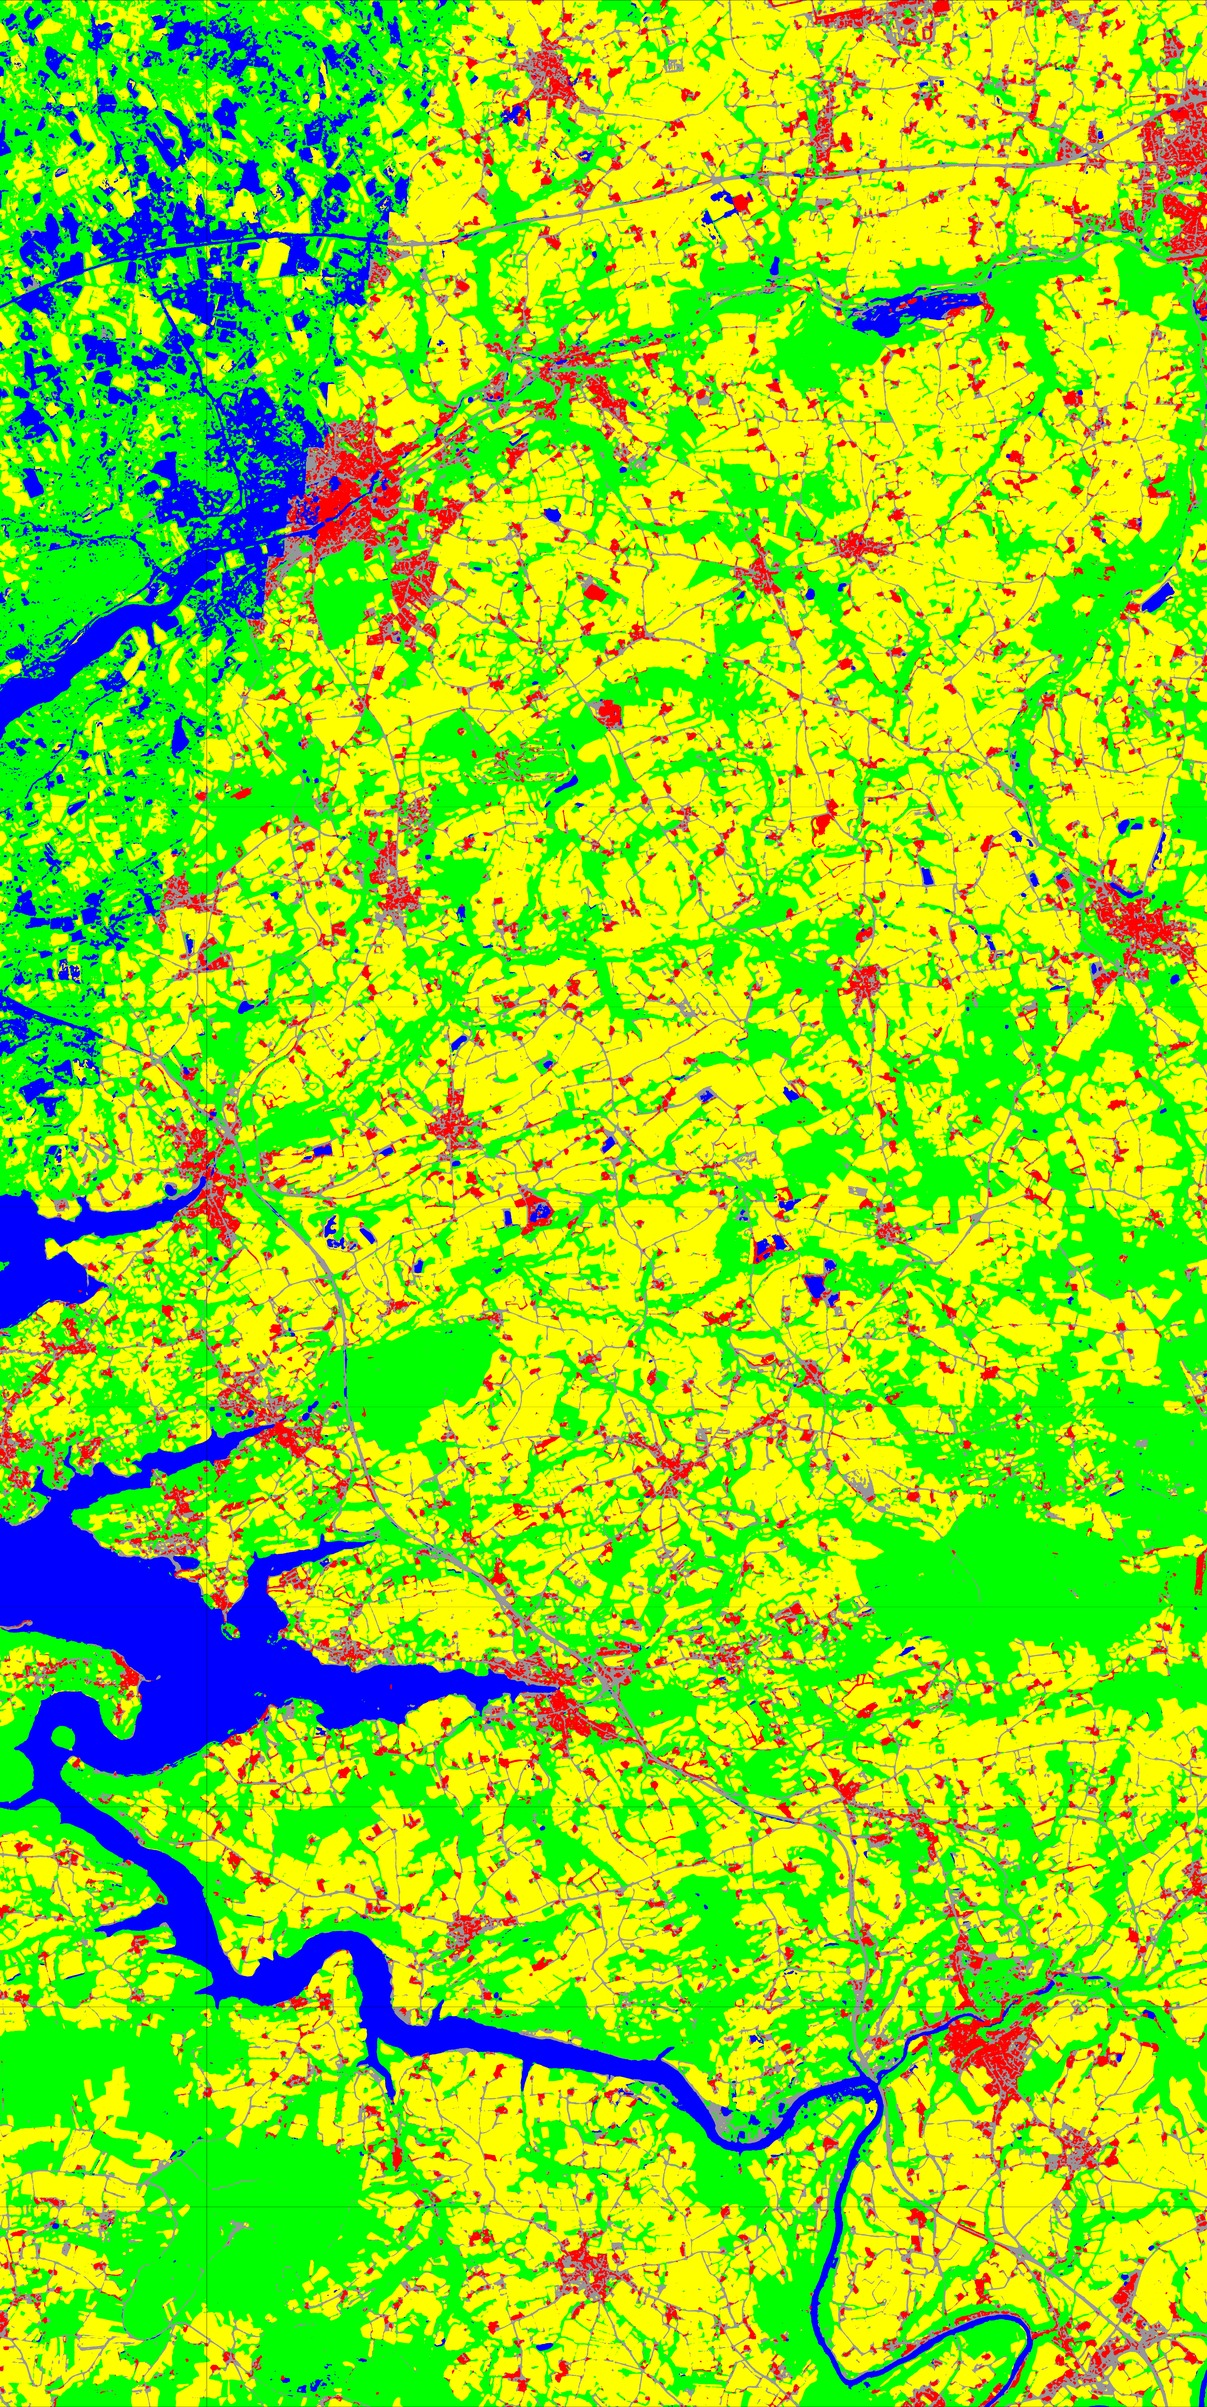
\includegraphics[width=\textwidth]{all_classif_S2}
        \caption{Sentinel-2}
    \end{subfigure}
    \begin{subfigure}{0.49\textwidth}
        \centering
        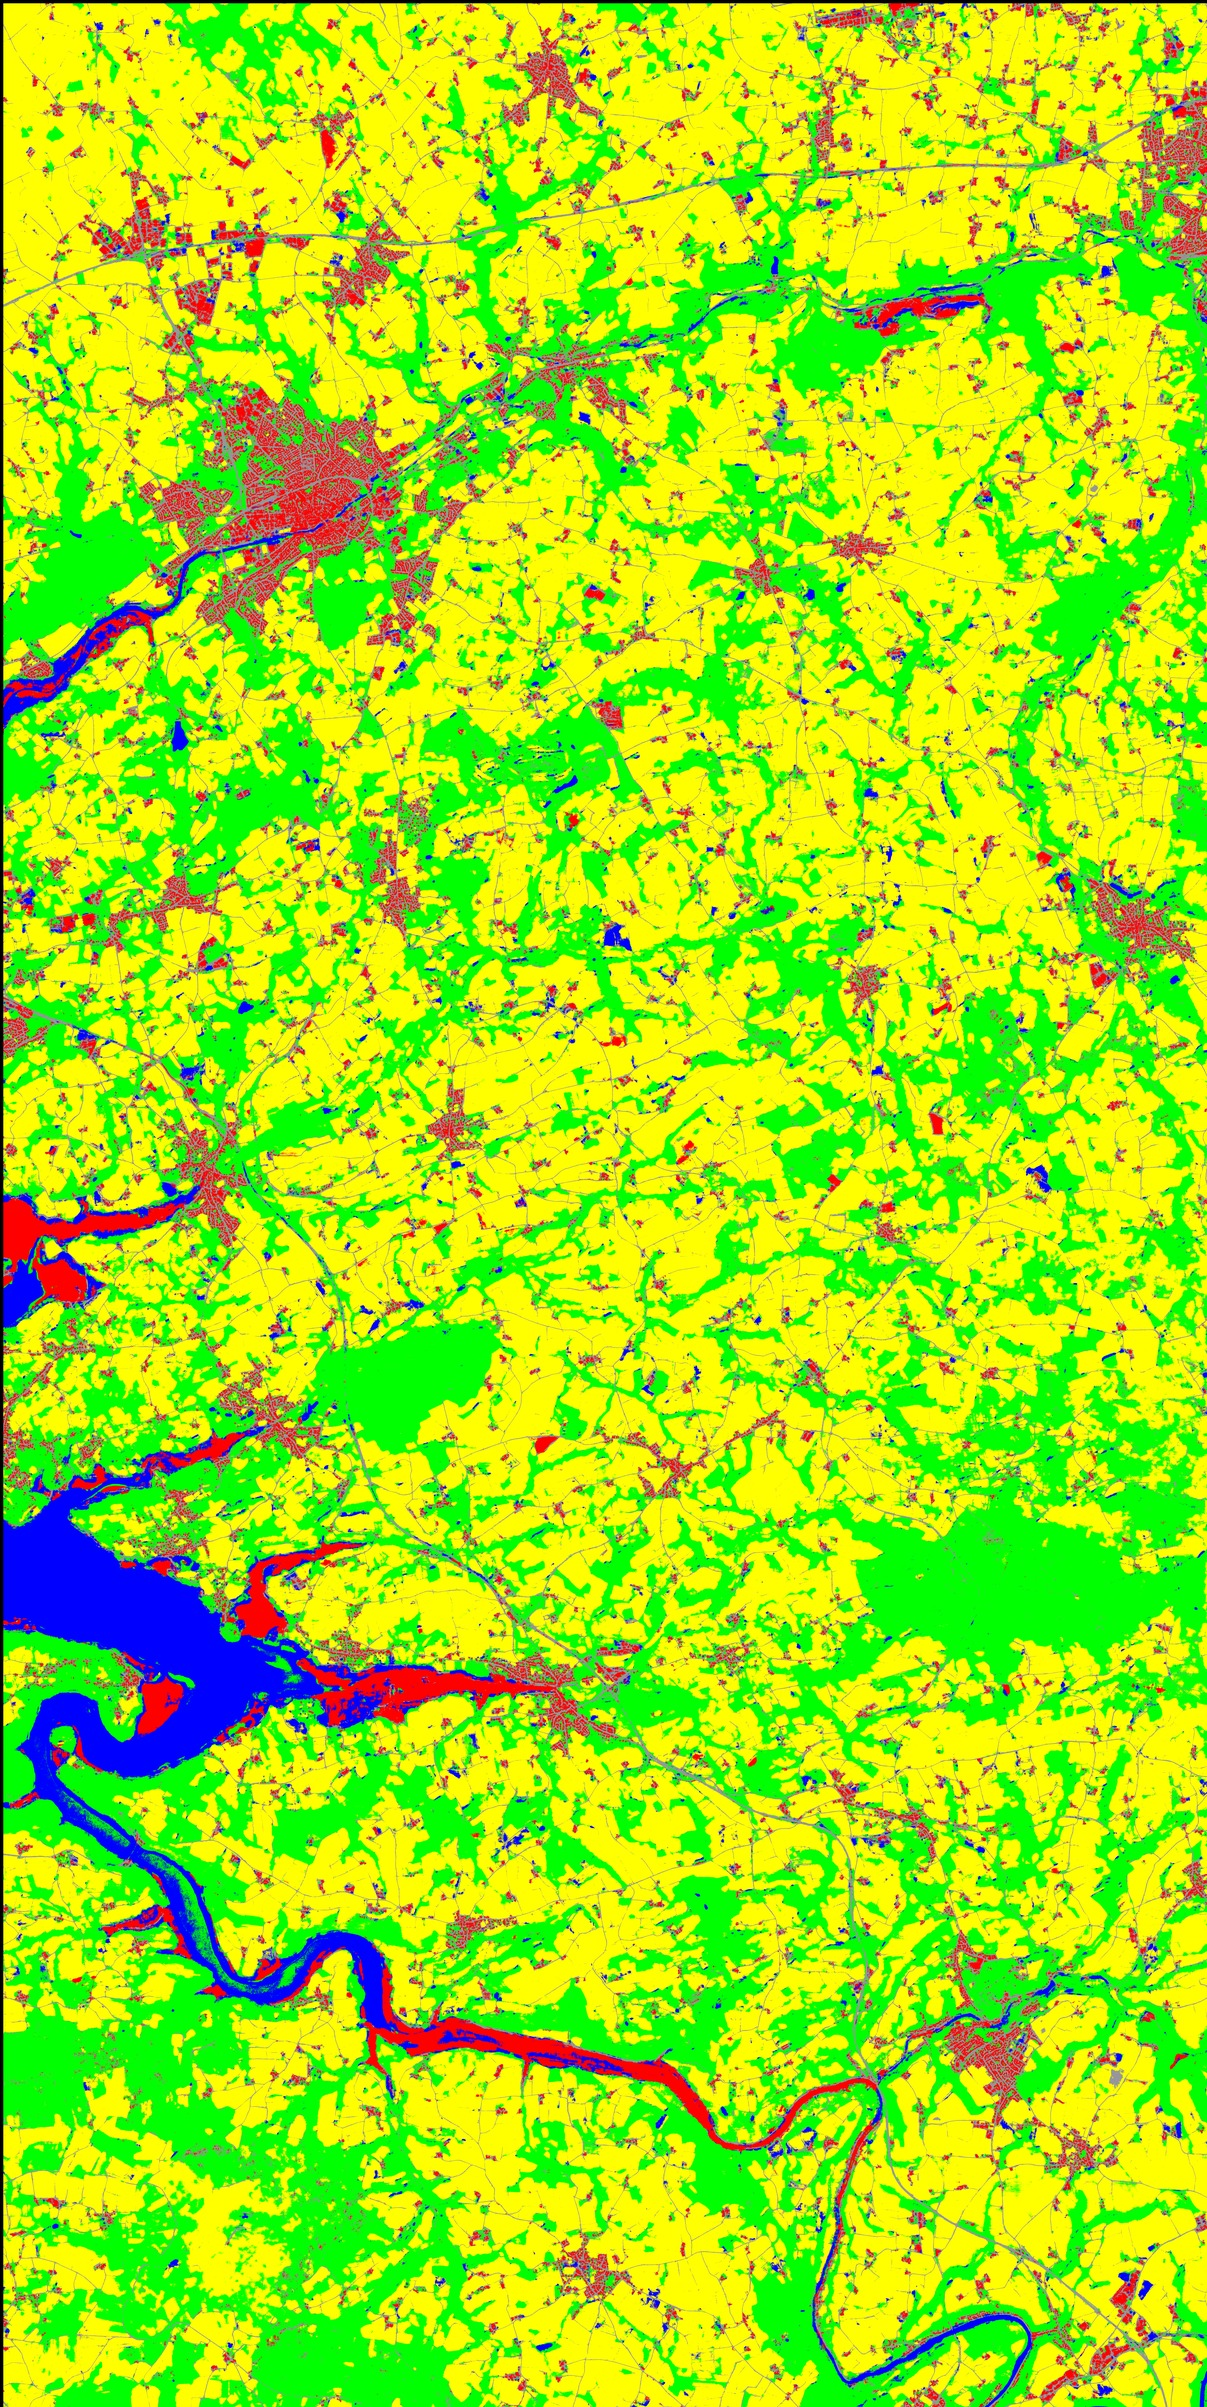
\includegraphics[width=\textwidth]{all_classif_SPOT6}
        \caption{SPOT6}
    \end{subfigure}
    \legende
    \caption{Initial classifications from Sentinel-2 and SPOT 6}
\end{figure}

\begin{figure}[H]
    \centering 
    \begin{subfigure}{0.49\textwidth}
        \centering
        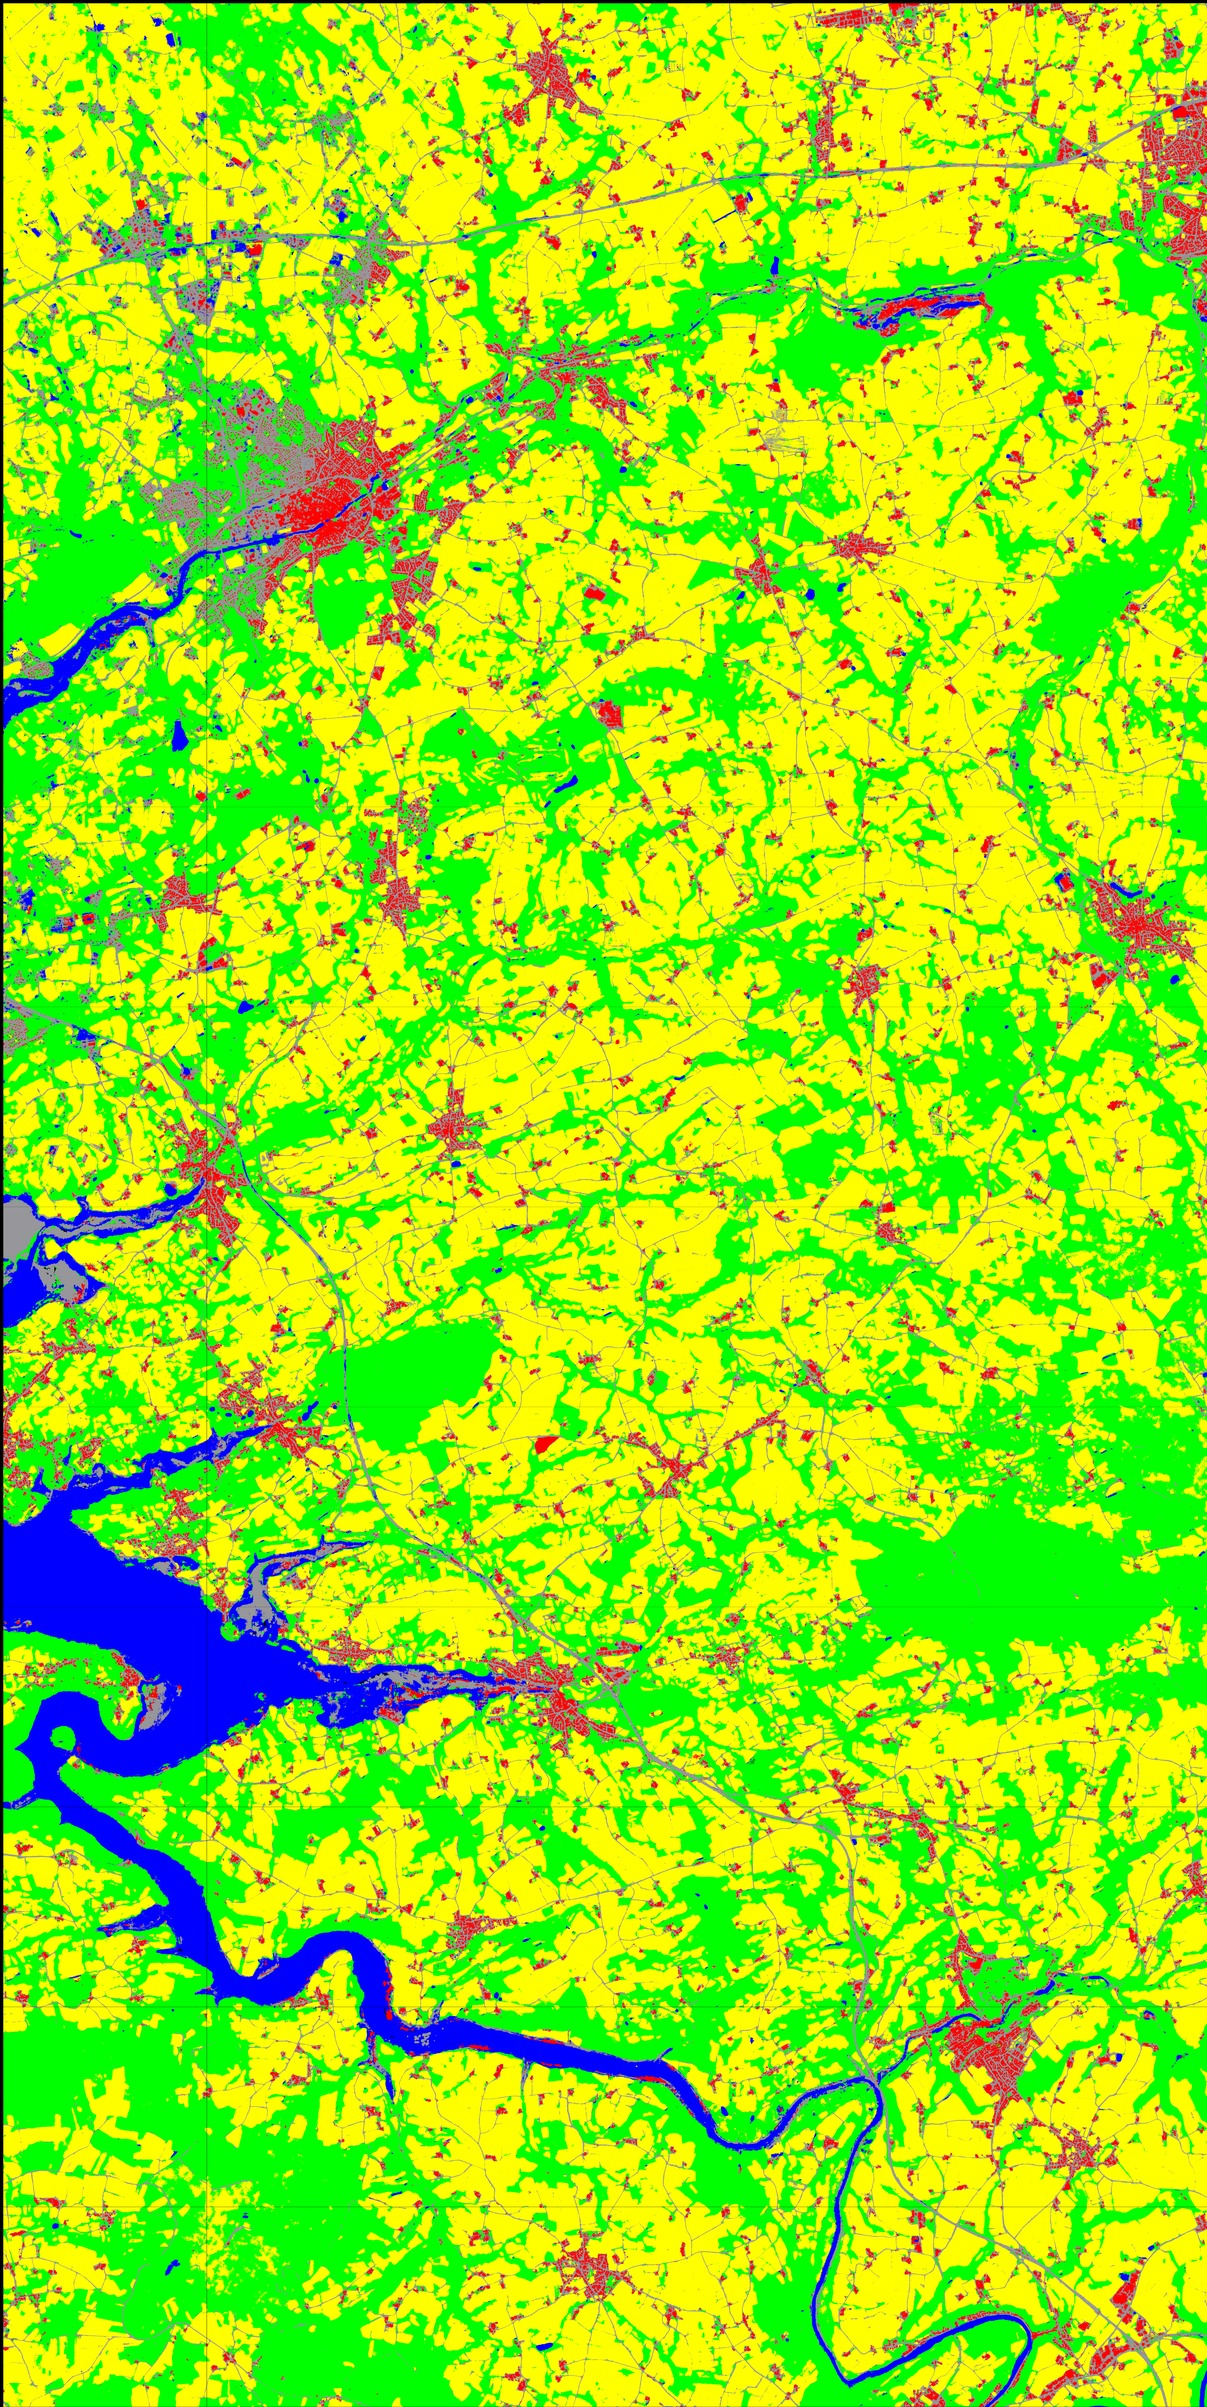
\includegraphics[width=\textwidth]{all_classif_Fusion_Min_weighted}
        \caption{Fusion (Min rule)}
    \end{subfigure}
    \begin{subfigure}{0.49\textwidth}
        \centering
        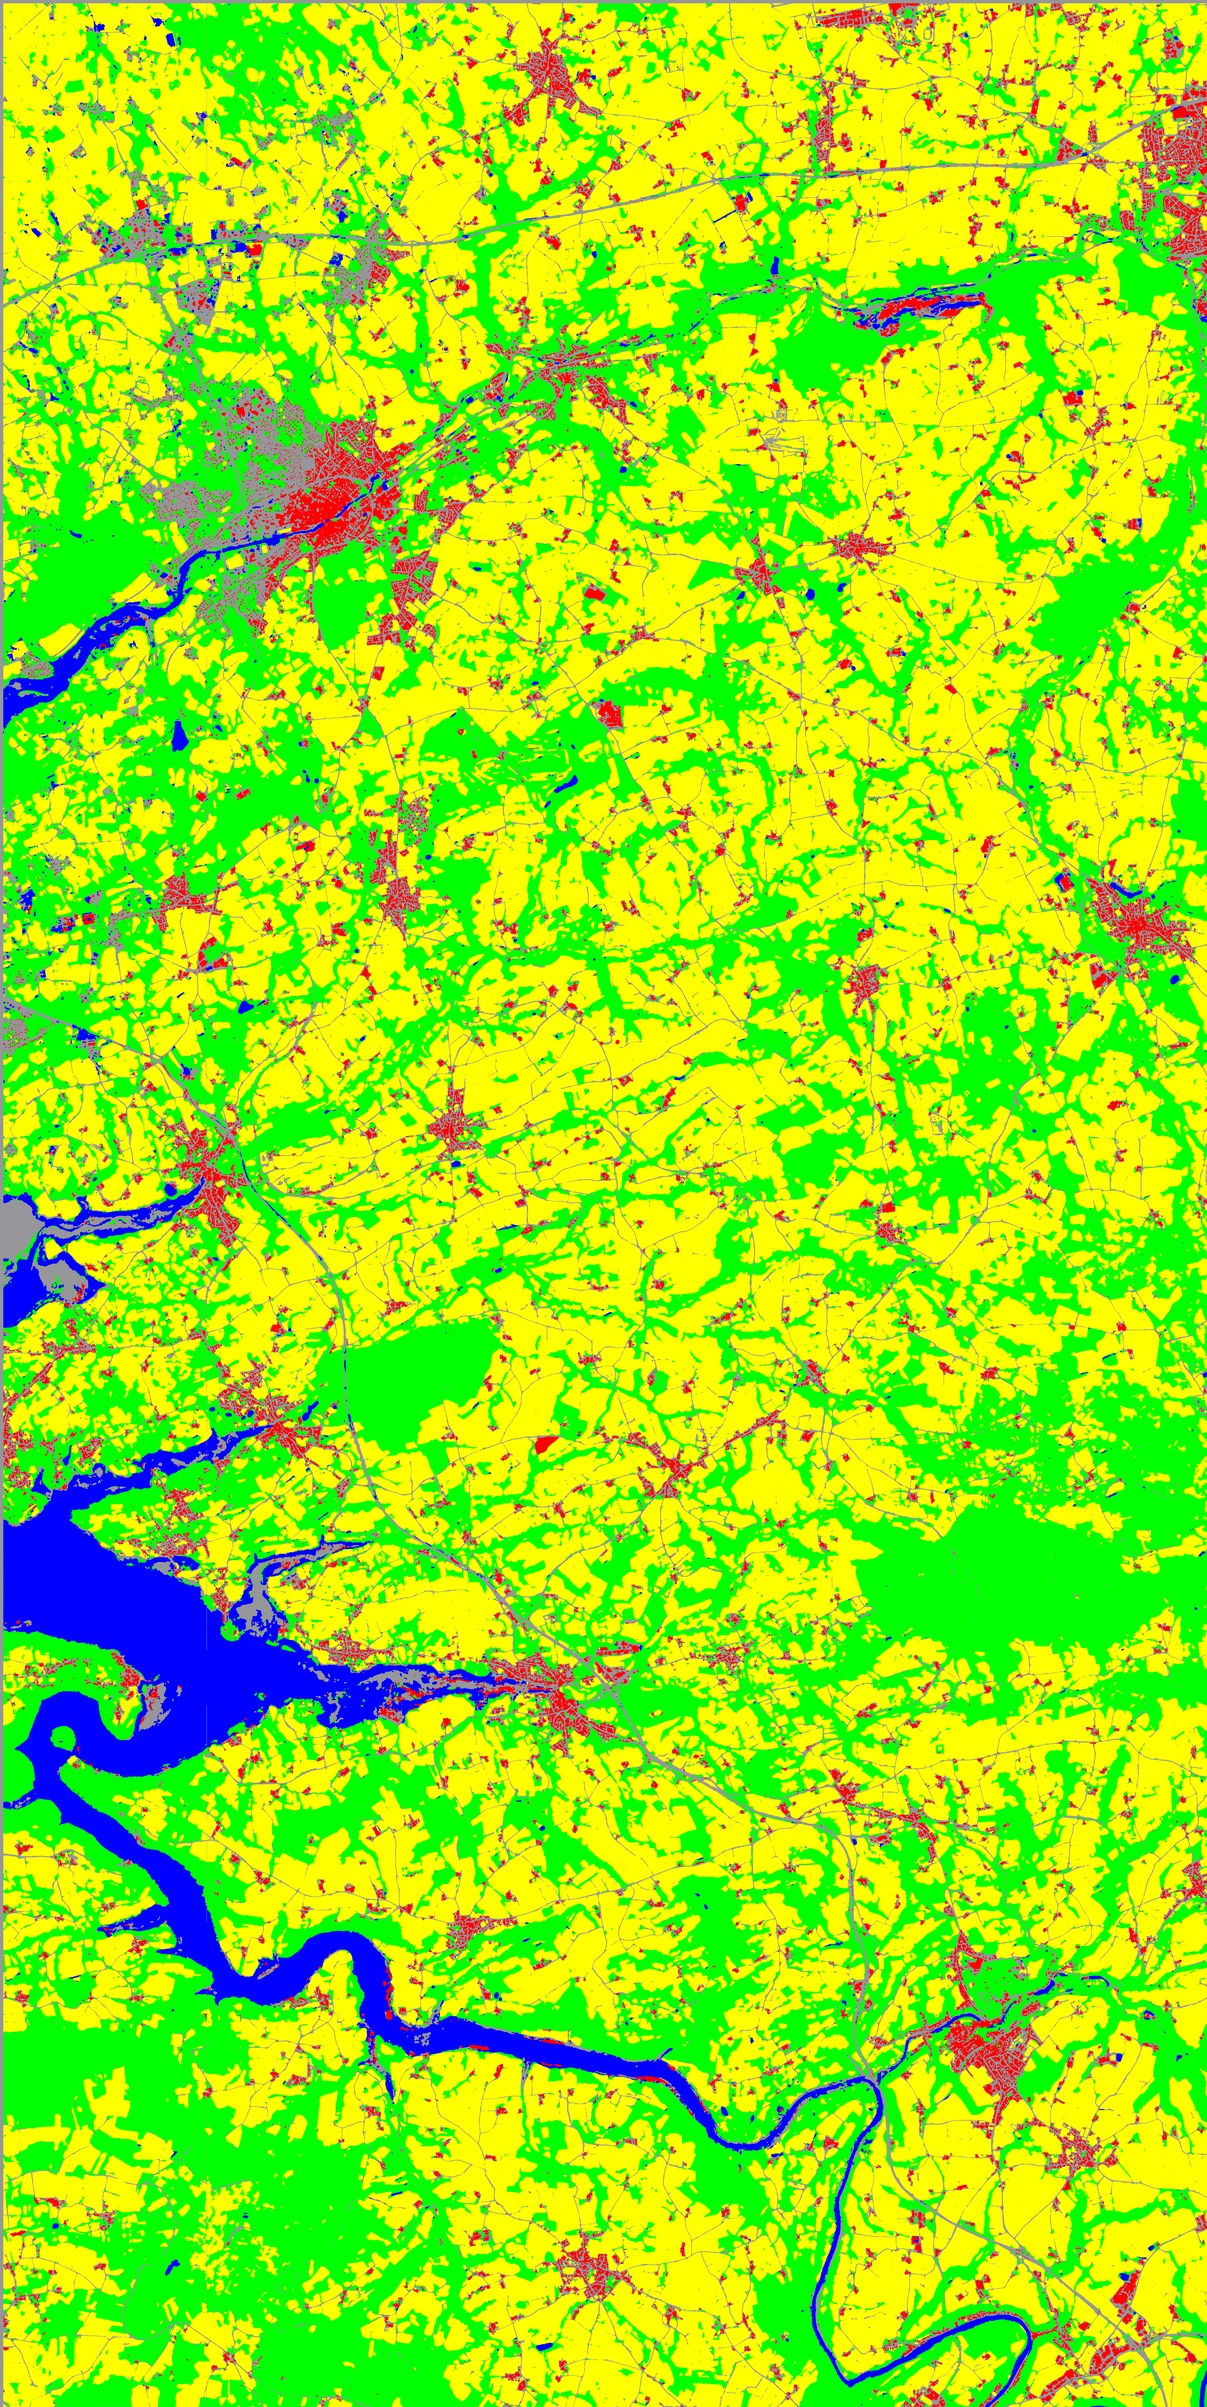
\includegraphics[width=\textwidth]{all_regul_Min_weighted_G2_l1000_g70_e500_0_0_0}
        \caption{Regularization} % parameters
    \end{subfigure}
    \legende
    \caption{Fusion and Regularization}
\end{figure}

\begin{figure}[H]
    \centering 
    \begin{subfigure}{0.49\textwidth}
        \centering
        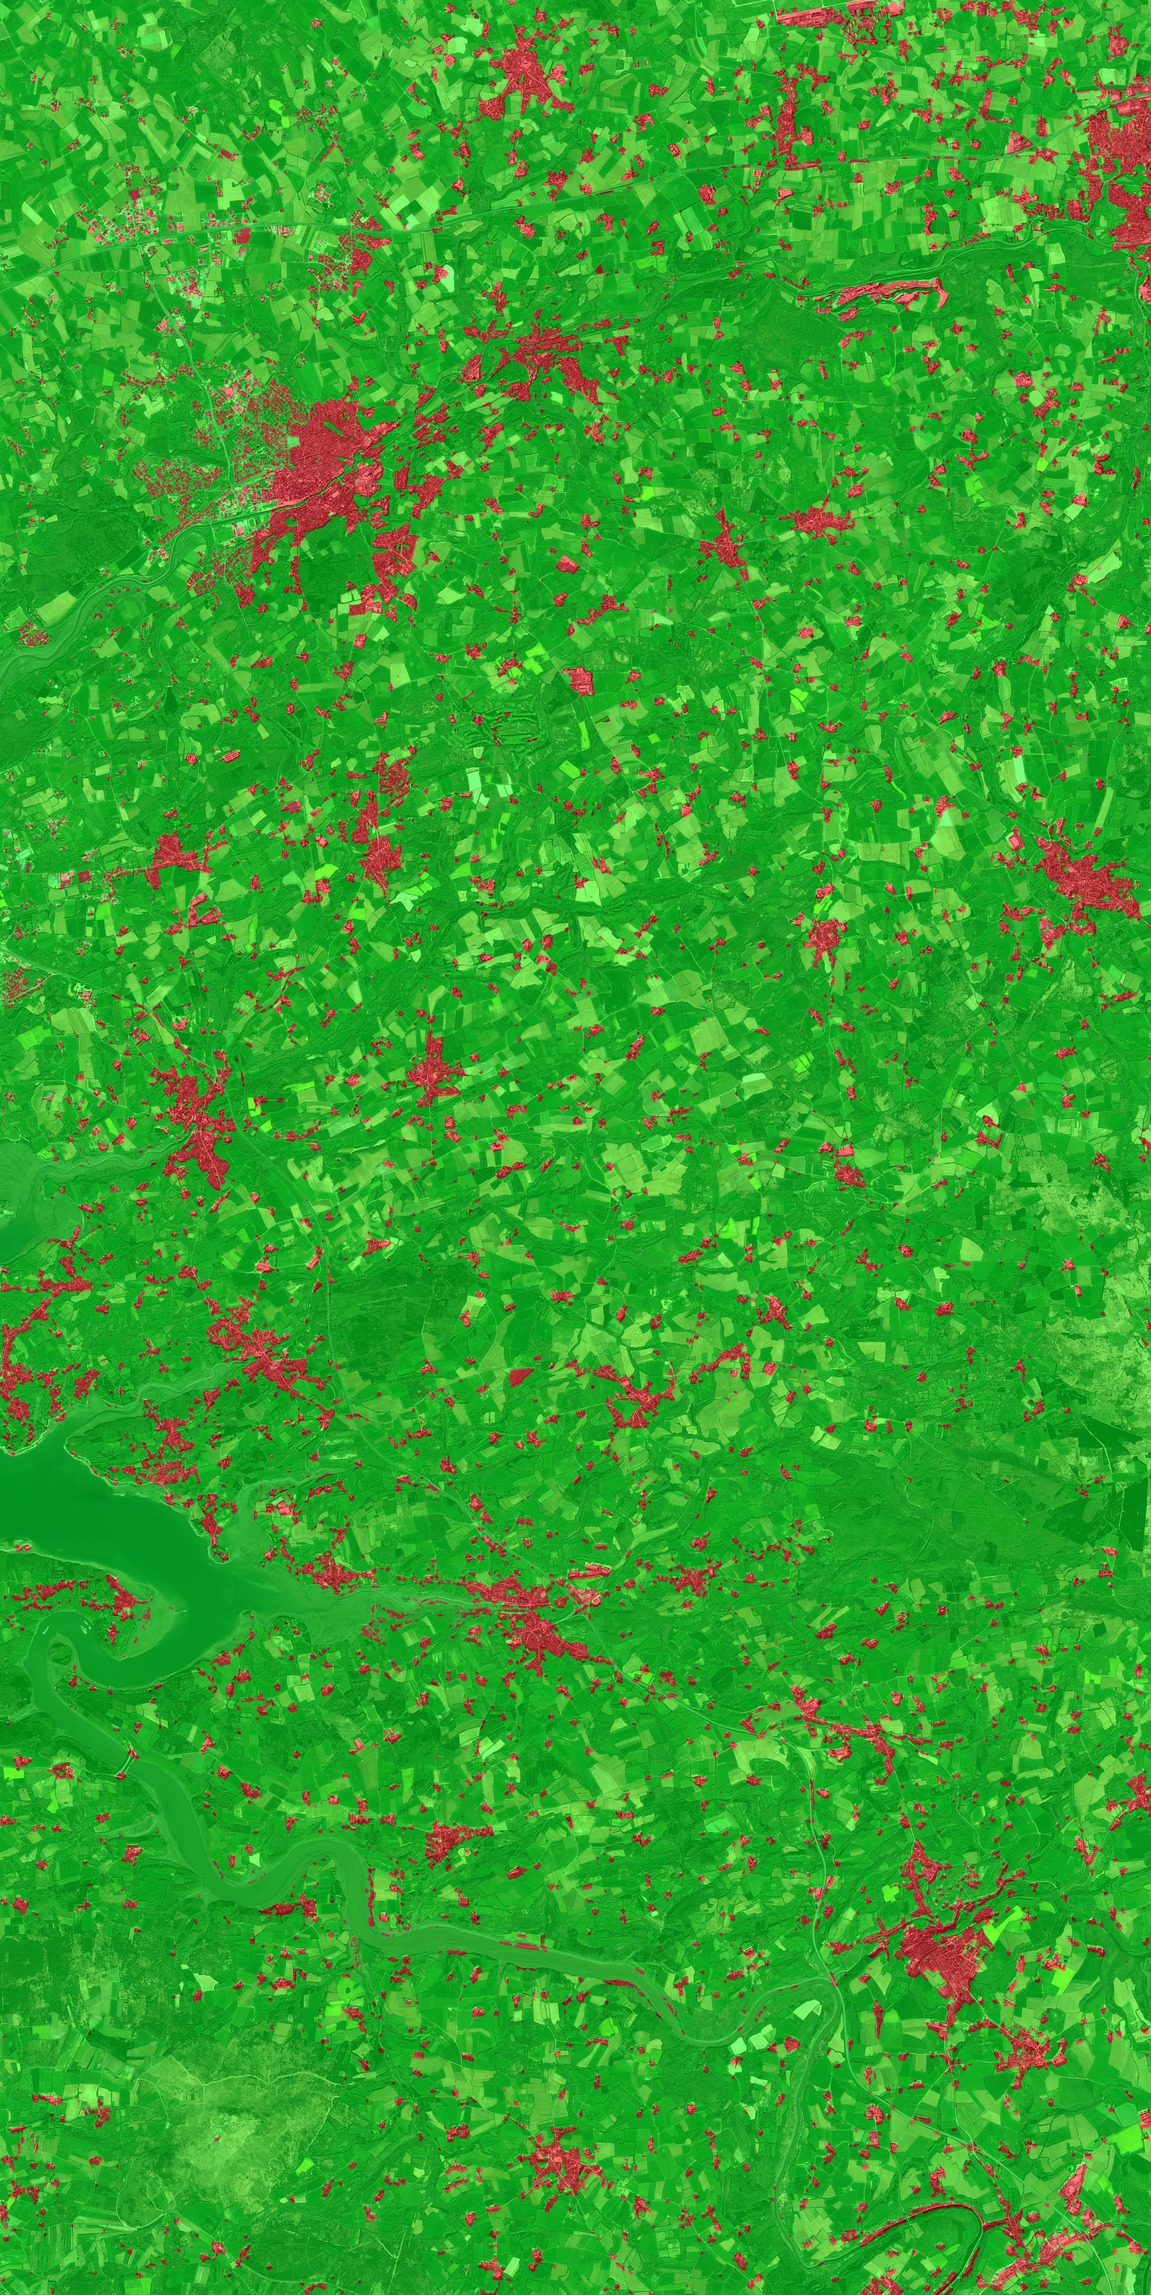
\includegraphics[width=\textwidth]{all_classif_Fusion_Min_overlay}
        \caption{Fusion (Min rule)}
    \end{subfigure}
    \begin{subfigure}{0.49\textwidth}
        \centering
        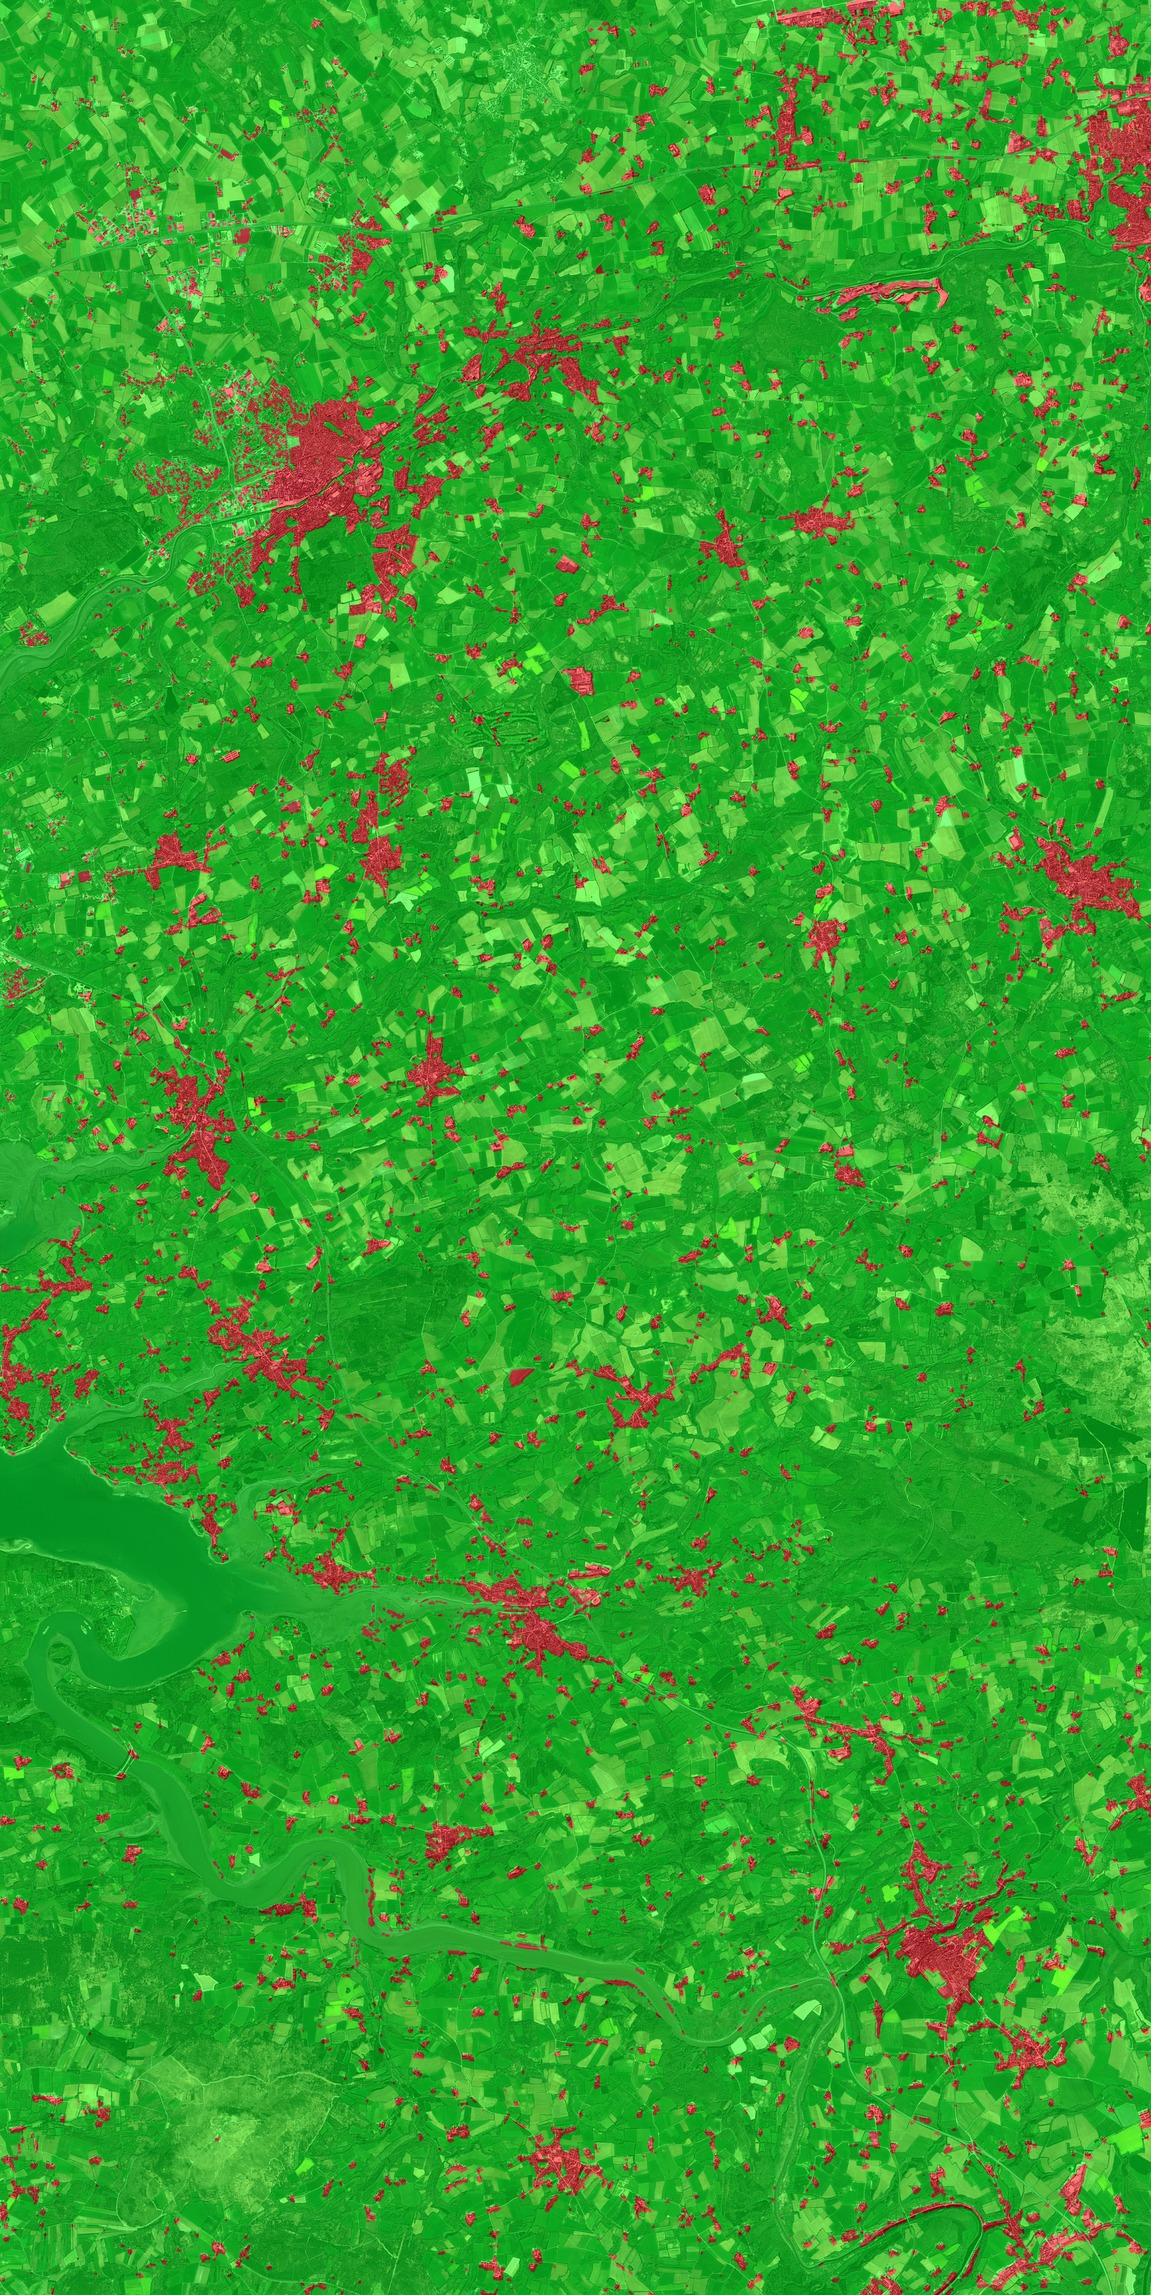
\includegraphics[width=\textwidth]{all_regul_Min_l1000_g30_e500_0_0_0_overlay}
        \caption{Regularization} % parameters
    \end{subfigure}
    \legendebin
    \caption{Second Fusion with S2 and Regularization}
\end{figure}
\begin{figure}[H]
    \centering 
    \foreach \n in {3,8}{
    \begin{subfigure}{0.49\textwidth}
        \centering
        \includegraphics[width=\textwidth]{all_regul_seg_maj_\n_overlay}
        \caption{cut=\n}
    \end{subfigure}
    }
    \legendebin
    \caption{Segmentation and majority vote (I)}
\end{figure}
\begin{figure}[H]
    \centering 
    \foreach \n in {20,30}{
    \begin{subfigure}{0.49\textwidth}
        \centering
        \includegraphics[width=\textwidth]{all_regul_seg_maj_\n_overlay}
        \caption{cut=\n}
    \end{subfigure}
    }
    \legendebin
    \caption{Segmentation and majority vote (II)}
\end{figure}
\restoregeometry
\end{appendices}   
\end{document}
\endinput